\documentclass[11pt,letterpaper]{article}
\usepackage[margin=1in]{geometry} % see geometry.pdf on how to lay out the page. There's lots.
\geometry{a4paper} % or letter or a5paper or ... etc
\usepackage{graphicx}
\usepackage{amsmath,amssymb}
\usepackage{natbib} \bibpunct{(}{)}{;}{author-year}{}{,} 
\usepackage[usenames,dvipsnames,svgnames,table]{xcolor}
\usepackage{color}
\usepackage{amssymb}
\usepackage{setspace}

%\usepackage[hidelinks]{hyperref}


\usepackage[normalem]{ulem}

\newcommand{\alisa}[1]{{\em \color{red} #1}}
\newcommand{\plr}[1]{{\em \color{blue} #1}}
\newcommand{\yb}[1]{{\em \color{magenta} #1}}

\newcommand{\E}{\mathbb{E}}
\renewcommand{\P}{\mathbb{P}}
\newcommand{\R}{\mathbb{R}}
\newcommand{\one}{\mathbf{1}}
\DeclareMathOperator{\sgn}{sgn}
\newcommand{\grad}{\nabla}

\newcommand{\deriv}[1]{\frac{d}{d#1}}
\newcommand{\dderiv}[1]{\frac{d^2}{d#1^2}}
\newcommand{\given}{\,\vert\,}
\newcommand{\st}{\,\colon\,}
\renewcommand{\and}{\,\&\,}


% doesn't work with hyperref
% \usepackage{xr}
% \externaldocument{supplement}

\usepackage{lineno}

% from http://tex.stackexchange.com/questions/43648/why-doesnt-lineno-number-a-paragraph-when-it-is-followed-by-an-align-equation/55297#55297
\newcommand*\patchAmsMathEnvironmentForLineno[1]{%
  \expandafter\let\csname old#1\expandafter\endcsname\csname #1\endcsname
  \expandafter\let\csname oldend#1\expandafter\endcsname\csname end#1\endcsname
  \renewenvironment{#1}%
     {\linenomath\csname old#1\endcsname}%
     {\csname oldend#1\endcsname\endlinenomath}}% 
\newcommand*\patchBothAmsMathEnvironmentsForLineno[1]{%
  \patchAmsMathEnvironmentForLineno{#1}%
  \patchAmsMathEnvironmentForLineno{#1*}}%
\AtBeginDocument{%
\patchBothAmsMathEnvironmentsForLineno{equation}%
\patchBothAmsMathEnvironmentsForLineno{align}%
\patchBothAmsMathEnvironmentsForLineno{flalign}%
\patchBothAmsMathEnvironmentsForLineno{alignat}%
\patchBothAmsMathEnvironmentsForLineno{gather}%
\patchBothAmsMathEnvironmentsForLineno{multline}%
}

% Responses to reviews
\usepackage{lineno}
% \usepackage[hypertexnames=false]{hyperref}   % not working correctly
% \usepackage{latexml}

\linenumbers


%%%%%  PUT THIS IN HEADER OF FILE
% % Responses to reviews:
% \usepackage{lineno}
% \usepackage[hypertexnames=false]{hyperref}   % not working correctly
% \usepackage{latexml}

\linenumbers


%%%%%  PUT THIS IN HEADER OF FILE
% % Responses to reviews:
% \usepackage{lineno}
% \usepackage[hypertexnames=false]{hyperref}   % not working correctly
% \usepackage{latexml}

\linenumbers


%%%%%  PUT THIS IN HEADER OF FILE
% % Responses to reviews:
% \input{review-response-commands}
% % set this to show line numbers and include responses to reviews or not
% \newif\ifreviewresponses
% \reviewresponsestrue  % include them
% % \reviewresponsesfalse  % don't include them
% \newcommand{\responsefile}{pbio-reviews-19sept12-responses.tex}  % name of the review reponses file

% counters for reviewer points
%% instead do reviewer labels
% \newcounter{reviewer}
% \setcounter{reviewer}{0}
\newcommand{\thereviewer}{}
\newcounter{point}
\setcounter{point}{0}

% pass in to \reviewersection the label for this reviewer (i.e. \reviewersection{1} or \reviewersection{AE})
\newcommand{\reviewersection}[1]{\renewcommand{\thereviewer}{#1}
                  \setcounter{point}{0}
                  \section*{Reviewer \thereviewer:}}
% drawing from from http://tex.stackexchange.com/questions/2317/latex-style-or-macro-for-detailed-response-to-referee-report
%% arguments to \point are (name of the point, optional) and (content)
\newenvironment{point}[1]
        { \refstepcounter{point} \bigskip \hrule \medskip \noindent 
                \slshape {\fontseries{b}\selectfont (\thereviewer.\thepoint) #1} }
        { }
\newcommand{\reply}{\normalfont \medskip \noindent \textbf{Reply}:\ }   

% use this command in the text where a change addressing a reviewer point has occurred
% e.g. \revpoint{1}{3} for reviewer 1, point 3
\newcommand{\revpoint}[2]{\linelabel{rr:rev#1:#2}}
% and this one to refer to such a location, e.g. \revreffull{1}{3}
\newcommand{\revreffull}[2]{{(p.\ \pageref{rr:rev#1:#2}, l.\ \lineref{rr:rev#1:#2})}}
% but this version fills in reviewer and point automatically if called in the appropriate part of the reviews
\newcommand{\revref}{\revreffull{\thereviewer}{\thepoint}}

% or, this one to refer to a named linelabel
% e.g. if in the text there is a \linelabel{approx_eqn_point}
% refer to it with \llname{approx_eqn_point}
\newcommand{\llname}[1]{{(p.\ \pageref{#1}, l.\ \lineref{#1})}}

% put this where the reviews are to appear (at the end?)
\newcommand{\includereviews}{
    \ifreviewresponses
    \clearpage
    \setcounter{page}{1}
    \setcounter{section}{0}
    \setcounter{subsection}{0}
    \nolinenumbers
    % \begin{center}
    %   {\LARGE \bf Response to Reviews}
    % \end{center}
    \input{\responsefile}
    \fi
}

% Useful shortcuts
\newcommand{\rollover}{ \reply{The reviewer makes an excellent point that we have missed out entirely.  We have made all the changes suggested, down to the minutiae \revref.} }
\newcommand{\playdead}{ \reply{The reviewer makes an excellent point.  We have made an utterly trivial change {\revref} that we think deals entirely with the concern raised.} }
                                                                                                         
% from http://tex.stackexchange.com/questions/43648/why-doesnt-lineno-number-a-paragraph-when-it-is-followed-by-an-align-equation/55297#55297
\ifcsname{patchAmsMathEnvironmentForLineno}\endcsname
    \newcommand*\patchAmsMathEnvironmentForLineno[1]{%                                                       
      \expandafter\let\csname old#1\expandafter\endcsname\csname #1\endcsname                                
      \expandafter\let\csname oldend#1\expandafter\endcsname\csname end#1\endcsname                          
      \renewenvironment{#1}%                                                                                 
         {\linenomath\csname old#1\endcsname}%                                                               
         {\csname oldend#1\endcsname\endlinenomath}}%                                                        
    \newcommand*\patchBothAmsMathEnvironmentsForLineno[1]{%                                                  
      \patchAmsMathEnvironmentForLineno{#1}%                                                                 
      \patchAmsMathEnvironmentForLineno{#1*}}%                                                               
    \AtBeginDocument{%                                                                                       
    \patchBothAmsMathEnvironmentsForLineno{equation}%                                                        
    \patchBothAmsMathEnvironmentsForLineno{align}%                                                           
    \patchBothAmsMathEnvironmentsForLineno{flalign}%                                                         
    \patchBothAmsMathEnvironmentsForLineno{alignat}%                                                         
    \patchBothAmsMathEnvironmentsForLineno{gather}%                                                          
    \patchBothAmsMathEnvironmentsForLineno{multline}%                                                        
\fi

% % set this to show line numbers and include responses to reviews or not
% \newif\ifreviewresponses
% \reviewresponsestrue  % include them
% % \reviewresponsesfalse  % don't include them
% \newcommand{\responsefile}{pbio-reviews-19sept12-responses.tex}  % name of the review reponses file

% counters for reviewer points
%% instead do reviewer labels
% \newcounter{reviewer}
% \setcounter{reviewer}{0}
\newcommand{\thereviewer}{}
\newcounter{point}
\setcounter{point}{0}

% pass in to \reviewersection the label for this reviewer (i.e. \reviewersection{1} or \reviewersection{AE})
\newcommand{\reviewersection}[1]{\renewcommand{\thereviewer}{#1}
                  \setcounter{point}{0}
                  \section*{Reviewer \thereviewer:}}
% drawing from from http://tex.stackexchange.com/questions/2317/latex-style-or-macro-for-detailed-response-to-referee-report
%% arguments to \point are (name of the point, optional) and (content)
\newenvironment{point}[1]
        { \refstepcounter{point} \bigskip \hrule \medskip \noindent 
                \slshape {\fontseries{b}\selectfont (\thereviewer.\thepoint) #1} }
        { }
\newcommand{\reply}{\normalfont \medskip \noindent \textbf{Reply}:\ }   

% use this command in the text where a change addressing a reviewer point has occurred
% e.g. \revpoint{1}{3} for reviewer 1, point 3
\newcommand{\revpoint}[2]{\linelabel{rr:rev#1:#2}}
% and this one to refer to such a location, e.g. \revreffull{1}{3}
\newcommand{\revreffull}[2]{{(p.\ \pageref{rr:rev#1:#2}, l.\ \lineref{rr:rev#1:#2})}}
% but this version fills in reviewer and point automatically if called in the appropriate part of the reviews
\newcommand{\revref}{\revreffull{\thereviewer}{\thepoint}}

% or, this one to refer to a named linelabel
% e.g. if in the text there is a \linelabel{approx_eqn_point}
% refer to it with \llname{approx_eqn_point}
\newcommand{\llname}[1]{{(p.\ \pageref{#1}, l.\ \lineref{#1})}}

% put this where the reviews are to appear (at the end?)
\newcommand{\includereviews}{
    \ifreviewresponses
    \clearpage
    \setcounter{page}{1}
    \setcounter{section}{0}
    \setcounter{subsection}{0}
    \nolinenumbers
    % \begin{center}
    %   {\LARGE \bf Response to Reviews}
    % \end{center}
    \input{\responsefile}
    \fi
}

% Useful shortcuts
\newcommand{\rollover}{ \reply{The reviewer makes an excellent point that we have missed out entirely.  We have made all the changes suggested, down to the minutiae \revref.} }
\newcommand{\playdead}{ \reply{The reviewer makes an excellent point.  We have made an utterly trivial change {\revref} that we think deals entirely with the concern raised.} }
                                                                                                         
% from http://tex.stackexchange.com/questions/43648/why-doesnt-lineno-number-a-paragraph-when-it-is-followed-by-an-align-equation/55297#55297
\ifcsname{patchAmsMathEnvironmentForLineno}\endcsname
    \newcommand*\patchAmsMathEnvironmentForLineno[1]{%                                                       
      \expandafter\let\csname old#1\expandafter\endcsname\csname #1\endcsname                                
      \expandafter\let\csname oldend#1\expandafter\endcsname\csname end#1\endcsname                          
      \renewenvironment{#1}%                                                                                 
         {\linenomath\csname old#1\endcsname}%                                                               
         {\csname oldend#1\endcsname\endlinenomath}}%                                                        
    \newcommand*\patchBothAmsMathEnvironmentsForLineno[1]{%                                                  
      \patchAmsMathEnvironmentForLineno{#1}%                                                                 
      \patchAmsMathEnvironmentForLineno{#1*}}%                                                               
    \AtBeginDocument{%                                                                                       
    \patchBothAmsMathEnvironmentsForLineno{equation}%                                                        
    \patchBothAmsMathEnvironmentsForLineno{align}%                                                           
    \patchBothAmsMathEnvironmentsForLineno{flalign}%                                                         
    \patchBothAmsMathEnvironmentsForLineno{alignat}%                                                         
    \patchBothAmsMathEnvironmentsForLineno{gather}%                                                          
    \patchBothAmsMathEnvironmentsForLineno{multline}%                                                        
\fi

% % set this to show line numbers and include responses to reviews or not
% \newif\ifreviewresponses
% \reviewresponsestrue  % include them
% % \reviewresponsesfalse  % don't include them
% \newcommand{\responsefile}{pbio-reviews-19sept12-responses.tex}  % name of the review reponses file

% counters for reviewer points
%% instead do reviewer labels
% \newcounter{reviewer}
% \setcounter{reviewer}{0}
\newcommand{\thereviewer}{}
\newcounter{point}
\setcounter{point}{0}

% pass in to \reviewersection the label for this reviewer (i.e. \reviewersection{1} or \reviewersection{AE})
\newcommand{\reviewersection}[1]{\renewcommand{\thereviewer}{#1}
                  \setcounter{point}{0}
                  \section*{Reviewer \thereviewer:}}
% drawing from from http://tex.stackexchange.com/questions/2317/latex-style-or-macro-for-detailed-response-to-referee-report
%% arguments to \point are (name of the point, optional) and (content)
\newenvironment{point}[1]
        { \refstepcounter{point} \bigskip \hrule \medskip \noindent 
                \slshape {\fontseries{b}\selectfont (\thereviewer.\thepoint) #1} }
        { }
\newcommand{\reply}{\normalfont \medskip \noindent \textbf{Reply}:\ }   

% use this command in the text where a change addressing a reviewer point has occurred
% e.g. \revpoint{1}{3} for reviewer 1, point 3
\newcommand{\revpoint}[2]{\linelabel{rr:rev#1:#2}}
% and this one to refer to such a location, e.g. \revreffull{1}{3}
\newcommand{\revreffull}[2]{{(p.\ \pageref{rr:rev#1:#2}, l.\ \lineref{rr:rev#1:#2})}}
% but this version fills in reviewer and point automatically if called in the appropriate part of the reviews
\newcommand{\revref}{\revreffull{\thereviewer}{\thepoint}}

% or, this one to refer to a named linelabel
% e.g. if in the text there is a \linelabel{approx_eqn_point}
% refer to it with \llname{approx_eqn_point}
\newcommand{\llname}[1]{{(p.\ \pageref{#1}, l.\ \lineref{#1})}}

% put this where the reviews are to appear (at the end?)
\newcommand{\includereviews}{
    \ifreviewresponses
    \clearpage
    \setcounter{page}{1}
    \setcounter{section}{0}
    \setcounter{subsection}{0}
    \nolinenumbers
    % \begin{center}
    %   {\LARGE \bf Response to Reviews}
    % \end{center}
    \input{\responsefile}
    \fi
}

% Useful shortcuts
\newcommand{\rollover}{ \reply{The reviewer makes an excellent point that we have missed out entirely.  We have made all the changes suggested, down to the minutiae \revref.} }
\newcommand{\playdead}{ \reply{The reviewer makes an excellent point.  We have made an utterly trivial change {\revref} that we think deals entirely with the concern raised.} }
                                                                                                         
% from http://tex.stackexchange.com/questions/43648/why-doesnt-lineno-number-a-paragraph-when-it-is-followed-by-an-align-equation/55297#55297
\ifcsname{patchAmsMathEnvironmentForLineno}\endcsname
    \newcommand*\patchAmsMathEnvironmentForLineno[1]{%                                                       
      \expandafter\let\csname old#1\expandafter\endcsname\csname #1\endcsname                                
      \expandafter\let\csname oldend#1\expandafter\endcsname\csname end#1\endcsname                          
      \renewenvironment{#1}%                                                                                 
         {\linenomath\csname old#1\endcsname}%                                                               
         {\csname oldend#1\endcsname\endlinenomath}}%                                                        
    \newcommand*\patchBothAmsMathEnvironmentsForLineno[1]{%                                                  
      \patchAmsMathEnvironmentForLineno{#1}%                                                                 
      \patchAmsMathEnvironmentForLineno{#1*}}%                                                               
    \AtBeginDocument{%                                                                                       
    \patchBothAmsMathEnvironmentsForLineno{equation}%                                                        
    \patchBothAmsMathEnvironmentsForLineno{align}%                                                           
    \patchBothAmsMathEnvironmentsForLineno{flalign}%                                                         
    \patchBothAmsMathEnvironmentsForLineno{alignat}%                                                         
    \patchBothAmsMathEnvironmentsForLineno{gather}%                                                          
    \patchBothAmsMathEnvironmentsForLineno{multline}%                                                        
\fi

% set this to show line numbers and include responses to reviews or not
\newif\ifreviewresponses
\reviewresponsestrue  % include them
% \reviewresponsesfalse  % don't include them
\newcommand{\responsefile}{review-responses-april-2016.tex}  % name of the review reponses file


% other title ideas:
% {Blocks of extended ancestry around selected loci in hybrid zones}
\title{Beyond clines: lineages and haplotype blocks in hybrid zones}
\author{}
\date{} % delete this line to display the current date

\usepackage{authblk}

\usepackage[hidelinks]{hyperref}
\AtBeginDocument{\let\textlabel\label}

\begin{document}

\thispagestyle{empty}
\author[*]{Alisa Sedghifar}
\author[$\S$]{Yaniv Brandvain}
\author[$\dag$]{Peter Ralph}



\affil[*]{\small{Lewis-Sigler Institute for Integrative Genomics and Department of Ecology and Evolutionary Biology, Princeton University, Princeton, New Jersey, 08544}}
%\affil[2]{Department of Evolution and Ecology, University of California, Davis, Davis, California, United Sates of America}
\affil[$\S$]{\small{Department of Plant Biology, University of Minnesota, St.~Paul, Minnesota, 55108}}
\affil[$\dag$]{\small{Department of Molecular and Computational Biology, University of Southern California, Los Angeles, California, 90089}}

%%% BEGIN DOCUMENT

\maketitle
%\tableofcontents


\abstract{
Hybrid zones formed between recently diverged populations offer an opportunity 
to study the mechanisms underlying reproductive isolation and the process of speciation.
Here, we use a combination of analytical theory and explicit forward simulations
to describe how selection against hybrid genotypes impacts patterns of introgression
across genomic and geographic space. 
By describing how lineages move across the hybrid zone, in a model without coalescence, 
we add to modern understanding of how clines form and how parental haplotypes are broken up during introgression.
Working with lineages makes it easy to see that
clines form in about $1/s$ generations, where $s$ is the strength of selection against hybrids,
and linked clines persist over a genomic scale of $1/T$, where $T$ is the age, in generations, of the hybrid zone. 
Locally disadvantageous alleles tend to exist as small families,
whose lineages trace back to the side from which they originated at speed $\sqrt{s}$ dispersal distances per generation.
The lengths of continuous tracts of ancestry provide an additional source of information:
blocks of ancestry surrounding single-locus incompatibilities can be substantially longer than the genome-wide average block length at the same spatial location,
an observation that might be used to characterize the age of hybrid zones
and identify candidate targets of selection.
%\alisa{ascertainment bias. Tract lengths provide additional source of information, as they provide unbiased information even when used ascertained markers.}

\textbf{Keywords:} hybridization, tension zone, introgression, haplotypes, diffusion methods.
}

\linenumbers
\doublespacing


%%%%% %%%%%% %%%%%%%
\section*{Introduction}

% summary of intro:
%  clines happen
%  but then decay unless selection
%  which affects haplotypes and LD
%  most work so far just looks at clines
%  but haplotype blocks should be helpful
%  here we look at that stuff

The process of speciation commonly involves populations diverging with relatively little gene flow \citep{Coyne2004}.  
However, when formerly isolated populations come into contact before reproductive isolation is complete, some gene flow is possible.
Interbreeding and migration between such populations  
creates a gradient of alleles derived from the two populations across geographic space,
centered on their point of contact \citep[reviewed by][]{Barton1985}. 
If the populations are sufficiently diverged, 
this process leaves a distinct pattern of variation across the genome, 
in which long tracts of divergent haplotypes from each ancestral population  
are broken up by historical recombination events,
forming chromosomal {junctions} in ancestry \citep{Fisher1954, Chapman2002, baird2003distribution}. 
These patterns of correlated ancestry in admixed populations have been previously used to infer histories of hybridization and admixture 
\citep[e.g.,][]{Gravel2012,Hellenthal2014,Harris2013,sedghifar2015spatial}.

%The distribution of ancestry tract length in admixed or hybridizing populations has been used to infer the extent of hybridization and timing of secondary contact both in single populations and in hybrid zones \citep{Price2009, Gravel2012,sedghifar2015spatial}. In addition to allowing researchers to interpret non-equilibrium patterns of diversity in hybrid zones, 
%the length distribution of ancestry tracts could reveal the impact of ongoing selection on the mixing of ancestral genomes. %and, consequently, the maintenance of species distinctness. 
%In the extreme case of zero fitness in first-generation hybrids, for example, parental genomes will never mix and the stable hybrid zone will resemble a recently formed one. 
%If hybrids have non-zero fitness, some amount of introgression can occur, and the distribution of ancestry tract length in such populations has been used to infer the extent %of hybridization and timing of secondary contact \citep{Price2009, Gravel2012}. 

Our work here builds on the large body of theory describing tension zones 
and aims to describe \emph{transient} dynamics with a focus on \emph{haplotype} patterns.
% which may carry substantial information about the formation of recent zones.
To do this, we take the reverse-time perspective,
understanding the temporal dynamics of the system by describing how lineages tracing back from the hybrid zone
moveme across space, conditioning on the frequencies of the selected allele and following them as they recombine between selected backgrounds
\citep[similar to][]{hudson1988coalescent}.
Using a combination of theory and simulated hybrid zones, 
and extending the framework of \citet{sedghifar2015spatial},
we describe genome-wide patterns of coancestry 
as they relate to hybrid zone age, genetic distance from selected locus and geographic distance from hybrid zone center. 

% In other words, the arrangement of ancestral haplotype segments
% is shaped by the number of recombination events that have taken place between ancestral genotypes,
% and so the length distribution of such segments contains information about the age of the hybrid zone and the relative strength of selection affecting subsets of the genome. 
In particular, we examine how heterogeneous patterns of the ancestry length distribution across the genome 
may help identify putative targets of selection in hybridizing populations, 
providing another source of information in addition to gradients in allele frequencies used in current approaches \citep[e.g.,][]{Porter1997, Gompert2012}. 
Specifically, we find that selection against hybrid incompatibility loci changes the extent of correlated ancestry --- that is, 
because selection rapidly removes incompatible alleles from heterospecific genomes, hybrid incompatibilities will be surrounded by disproportionately long ancestry blocks.


If hybrid ancestry at a given locus is disfavored, migrant haplotypes containing the selected allele will be removed rapidly from the population, preventing introgression of surrounding genomic regions. We therefore expect a deficit of short blocks of foreign ancestry surrounding the selected locus, with this effect becoming more pronounced further away from the center of a hybrid zone. As a corollary to this, conditional on having the ancestry that is at lower frequency (that is, being on the `wrong' side of the hybrid zone), the length of unbroken ancestry surrounding the selected locus is expected to be relatively long when far away from the zone center.  
This is because an unfit haplotype is more likely to have been recently inherited from the other side of the hybrid zone, 
and therefore will not have as many ancestors of the locally common type as do neutral haplotypes. 
This reasoning is applicable to instances of both tension zones generated by intrinsic genetic incompatibilities, and ecotone models of extrinsic ecological selection (e.g., local adaptation).

We neglect genetic drift in our analytical results \revpoint{2}{9}
because of the well-known problems with spatial coalescence \citep{felsenstein1975pain,barton2002continuous}.
This should provide a good model for stochastic motion of a single lineage (our main focus),
but does not model correlations between lineages or non-Markovian dynamics of the lineages.
This approach is common to much theoretical work,
that studies the reaction-diffusion equations that govern the deterministic, high-density limit \citep[as in][]{Nagylaki1975},
or the discrete analogues \citep{hanson1966effects}. 
There is also substantial work on how clines are affected by genetic drift \citep{Slatkin1975,felsenstein1975genetic,Nagylaki1978,durrett2007width,barton2008effect,Polechova2011}.
Our simulation results (below) suggest that although genetic drift strongly affects local noisiness of the system,
it does not substantially influence our conclusions at the moderate population densities we examine,
perhaps because we study relatively short time-scales.
At much lower population densities, however, local extinction and recolonization may have a stronger effect. \linelabel{ll:much_lower_densities}

There is also substantial work
quantifying the barrier to gene flow caused by clines \citep{barton1979gene,barton1986effects,Barton2000}.
We aim to complement this work,
and to investigate a possible new approach for identifying genomic regions experiencing selection in hybrid zones.

%\citet{Slatkin1973} pointed out, in a far-reaching general analysis,
%that while the environment may determine the location of a cline,
%the fitness of the heterozygote will likely determine the shape of the cline,
%and \citet{barton1986barrier} show that \alisa{clines under several different forms of selection are similar in shape.}
%\plr{(What forms of selection?)}

% YB REMOVED
%While for much of the genome, gene flow will eventually erase 
%both geographic clines in ancestry and strong correlations in ancestry across linked markers, 
%subsets of the genome can maintain stable clines in ancestry if selection against migrant, or hybrid, genotypes impedes gene flow across the hybrid zone \citep{barton1979gene}. 
      % previously had wrong Barton '79 here
%Studies of hybrid zones have primarily been based on single-site statistics (e.g., clines),
%but the recent availability of dense genotype data in combination with linkage information 
%makes it now possible to use patterns of the block length distribution
%to better understand the processes operating in hybrid zones.

% \alisa{
% Population genetic modeling of hybrid zones has focused largely on the 
% equilibrium states of clines at selected loci \citep{Nagylaki1975,barton1979dynamics,barton1986barrier,Slatkin1973,Slatkin1975,may1975gene,Haldane1948}.  
% Since stronger selection reduces the amount of genetic mixing,
% these models predict the narrowest clines 
% (i.e., the most rapid changes in allele frequencies)
% at loci close to selected loci, and wider clines at less tightly linked loci.
% In particular \citet{barton1979gene,barton1986barrier} have described patterns of clinal variation at loci linked to targets of selection.  
% This provides some expectation for how selection shapes covariance in ancestry at a single locus over geographic space.
% Our aim here is to extend this to include expectations for how selection shapes covariance in ancestry across the genome.}



%%%%%%% %%%%%%%%% %%%%%%%%
\section*{Methods}

%%%%%%% %%%%%%%%% 
\subsection*{The Model}

We consider two isolated populations
--- labeled species $A$ and species $B$ ---   % yb: for consistency with the rest of the MS
that came into contact $T$ generations in the past.  
We will say that species $A$ was initially on the ``left'' of the zone of contact, which corresponds to spatial positions $x<0$.  
After contact, the populations live across continuous geographical space,
with random, local dispersal that we take to be Gaussian
(although this should not affect the conclusions if the true dispersal distribution is not too fat-tailed).

We model selection through a single, underdominant locus:
at this locus, there are two alleles, one corresponding to each of the ancestral populations.
Individuals who are heterozygous at this locus produce on average $1-s$ times as many offspring than either homozygote.
Although most selection in hybrid zones is likely more complex than this simple situation, 
previous work has shown that such models generate clines that are very similar to models of ecological selection or epistatic systems \citep{Kruuk1999,barton2000epistasis}, 
because selection on an allele depends on its marginal effect on fitness.
(More discussion of this point in the Discussion.) \linelabel{ll:all_clines_are_the_same}





As in \citet{sedghifar2015spatial}, we consider where the ancestors of modern-day individuals
fall across geography as we look further back towards the time of first contact.  
We say that a locus in a sampled individual is of \emph{ancestry} $A$ if it has been inherited from an ancestor of species $A$,
i.e., if its lineage traces back to a spatial position $x<0$  at the time of secondary contact.
A block of genome is of ancestry $A$ if every locus in it does the same; 
	this occurs if there is no recombination in this block, or if all lineages generated by recombination events 
	in this block trace back to the $A$ side. 
This process, in which recombination events cause such lineages to \emph{branch},
is illustrated in Figure~\ref{Fig:schematic}.
We say that a block of genome is on the $A$ \emph{background} if it is physically linked to an allele of ancestry $A$ at the selected locus;
if a block of ancestry $A$ includes the selected site then it is necessarily on the $A$ background.
Because the identity of the selected allele determines how selection acts on the haplotype,
and because linked alleles can only move between the $A$ and the $B$ background in heterozygotes, 
a key factor in these models is the density and fecundity of heterozygotes.


%%%%%%%%
\begin{figure}
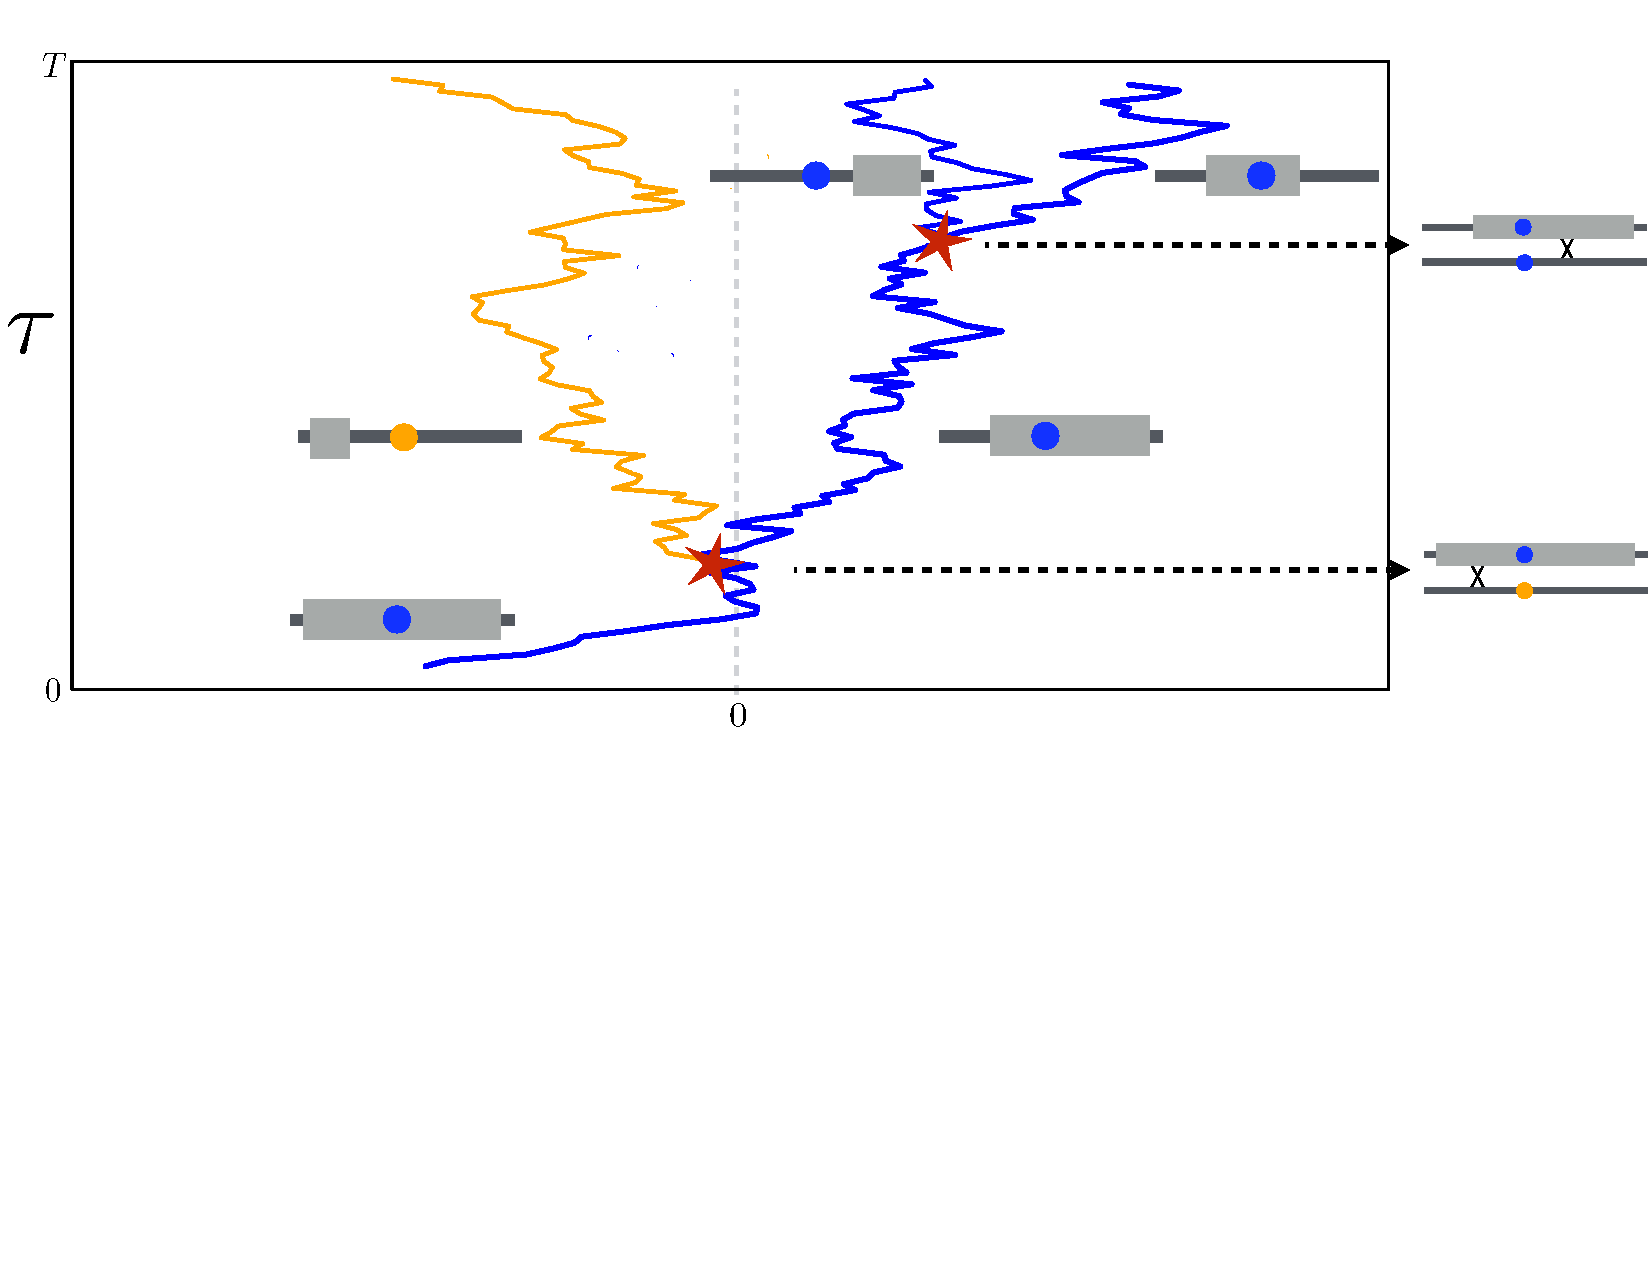
\includegraphics[clip,width=\textwidth,trim=0cm 8cm 0cm 0.05cm]{figs/BM_schematic_new2.pdf}
\caption{
    \textbf{A schematic figure of the lineages along which a segment of genome has been inherited,}
    showing the location (horizontal axis) and time (vertical axis) at which the ancestors 
    of a hypothetical sampled haplotype lived.
    At the time of sampling ($\tau=0$), the segment contains the $B$ allele at the selected locus.
    Paths traced by lineages across space are depicted by blue and yellow lines. 
    Branching events occur when there was a recombination event within the sampled segment.
    The rightmost blue line represents the path of the selected locus. 
    The colors of the other paths indicate the identity at the linked selected locus 
    (blue: linked to allele $B$; yellow: linked to allele $A$). 
    The center of the hybrid zone is at geographic position $x=0$; in the region $x<0$, ancestry $B$ is less common,
    and because of selection, the selected lineage spends little time there.
  %  Red dots represent ancestral recombination events that fall in the given segment of genome in an ancestor;
  %  these can cause the lineage to branch (lineages at linked sites are depicted as colored lines),
  %  or can switch lineages at linked sites between selected backgrounds 
  %  (yellow lineages are linked to the $A$ selected locus; blue are linked to $B$).
  %  Here the initial haplotype is broken up into 3 chunks over 100 generations,
  %  which switch between selected backgrounds once.
    Based on position of the lineages at $\tau=100$ generations ago,
    from left to right the segments are of ancestry $(A,B,B)$.
    % \plr{(Add blue/yellow bars at the bottom?)}
}\label{Fig:schematic}
\end{figure}


%%%%%%%% %%%%%%%%%%
\subsection*{Analysis}

In this section we aim to give both heuristics for how lineages move, 
that are helpful in providing intuition and for establishing order-of-magnitude estimates,
and analytics, mostly in terms of partial differential equations needing numerical solution. 

\paragraph{Establishment of the cline at the selected locus}
Deterministic theory predicts that after secondary contact,
the two alleles at the selected locus will form a stable cline,
affecting neighboring loci as well \citep{barton1979gene, barton1986barrier}.
First, we turn our attention to how the cline at the selected locus itself is formed.
%% we don't need to cite these here, since we cite Bazykin for the equation
% \alisa{Equations describing the forward-time establishment of the cline have been previously described \cite[e.g.,][]{Slatkin1973,may1975gene,Nagylaki1975}}
Write $p(x,t)$ for the frequency of the $A$ allele at spatial location $x$ and time $t$.  
Suppose that secondary contact occurred at time $t=0$, 
and the $A$ allele is initially fixed on the left, so
$p(x,0) = 1$ if $x<0$ and $p(x,0)=0$ if $x>0$.
% (In discrete computations, a deme at $x=0$ has $p(0,0)=1/2$.)
We assume that dispersal is local and unbiased;
and that the mean squared displacement between parent and offspring
in the direction perpendicular to the cline
is $\sigma^2$.
Assuming that: (i) alleles locally assort into diploids randomly, 
(ii) habitat and dispersal are homogeneous,
and (iii) population density is large,
% and (iv) $s$ and $\sigma$ are small, \alisa{relative to $N$ and $\tau$ respectively?}
then as in \citet{Bazykin1969},
the commonly-used equation that $p$ approximately solves is
\begin{align} \label{eqn:cline_pde}
    \frac{d}{dt} p = \frac{\sigma^2}{2} \frac{d^2}{dx^2} p +  2 p (1-p)  \times s (\frac{p}{2} - 1).
    %    \frac{d}{dt} p = \frac{\sigma^2}{2} \frac{d}{dx^2} p + s p (1-p) (2p-1) ,
\end{align}
Here the frequency $p=p(x,t)$ varies across time and space,
and so $ \frac{d}{dt} p$ is the local rate of change of the frequency of $A$.
The first term, $\frac{\sigma^2}{2} \frac{d^2}{dx^2} p$, describes the net rate at which $A$ alleles arrive by local dispersal.
The second term % ,  $2 p (1-p)  s (p/2-1)$,  % only need this term in the sentence once?
describes the impact of selection on local allele frequency as the product of local genotypic variance, $2p(1-p)$
(equivalently, the local frequency of heterozygotes), 
and selection on allele $A$, $s (p/2-1)$. 
The term $s (p/2-1)$ describes underdominance -- $A$ is favored when common ($p>1/2$) and disfavored when rare ($p<1/2$).
%YB: Pardon the extreme changes here, I tried to make things more obvious to a biologist
%and a logistic term proportional to the difference in reproductive rate between $A$ and $a$ alleles
%due to local proportions of heterozygotes,
%which is $s(2p-1)$ (up to an error of size $s^2$).
The equation can be derived as in \citet{Nagylaki1975};
the assumption of locally random mating was shown to have only a small effect \citet{christiansen1995genotypic}.

The equation is approximate because it 
omits terms of order $s^2$
(so deviations from the prediction occur over $1/s^2$ generations),
and relies on the Central Limit Theorem to approximate generation-to-generation dispersal by the Gaussian
(so if dispersal is non-Gaussian, will fit best over longer time scales, say, tens of generations).  \revpoint{AE}{2} 
As we show below, the solutions provide a good approximation across the range of realistic values of $s$.
Although there is no known exact analytic solution to this equation, 
the steady-state solution is
$\lim_{t \to \infty} p(x,t) = (1+\tanh(-2x\sqrt{s}/\sigma))/2$ \citep{Bazykin1969}. 
This relies on several approximations, but the general conclusions should be quite robust: 
the stable cline has width of order $\sigma/\sqrt{s}$, and decays exponentially. 

As noted by others \citep[e.g.,][]{Slatkin1973,may1975gene}, \linelabel{ll:rescaling}
rescaling space and time by $\sigma/\sqrt{s}$ and $1/s$ respectively in equation \eqref{eqn:cline_pde} 
results in a dimensionless equation,
implying that the cline establishes over a timescale of the order $1/s$. 
Since this is how long it takes diffusion at rate $\sigma^2$ to smooth across a region of width $\sigma/\sqrt{s}$,
this means we can think of
the cline as established by diffusion, 
despite being slowed down somewhat by selection against heterozygotes. 

For simplicity we mostly work with one-dimensional clines,
but the mathematics applies as well to two-dimensional systems with some modifications:
for instance, if the hybrid zone is a straight line, 
the description above applies to motion of a lineage transverse to the hybrid zone.  \revpoint{AE}{4}
In this case, $d^2/dx^2$ should be replaced by the Laplacian operator.
% and $d/dx$ by the gradient.
In fact, if the landscape is heterogeneous or dispersal is non-Gaussian,
the theory still holds replacing the Laplacian by the appropriate operator.
Note, however, that with low population densities, 
drift can have a strong effect that differs between one and two dimensional systems \citep{cox1995hybrid,barton2010phylogeography,durrett2007width}.


\paragraph{Lineages at the selected locus}
Now suppose that the frequency profile of the selected allele, $p(x,t)$, is known as a function of time and space.
We seek to first understand how lineages of sampled individuals behave at the selected locus,
and next extend the analysis to lineages at loci linked to the selected locus. 

Consider the collection of $A$ alleles found at geographic location $x$.
The expected number, among these alleles, that had a parent at location $y$ in the previous generation 
is proportional to the number of $A$ alleles that were at $y$ multiplied by the per-generation probability of dispersing from $y$ to $x$. 
In other words, lineages move as a random walk determined by the dispersal kernel,
but biased towards locations where the selected allele they carry is at higher frequency.
% (Lineages are also biased towards regions with higher fecundity,
% and thus away from the hybrid zone, but we assume that $s$ is small and ignore this.) 
% \alisa{could this reference to small $s$ be confusing?}
% \plr{it's confusing because it's differences in fecundity that bias the lineage since they create the net flux of A alleles to the right, even though there's a different term in how a lineage moves for the difference in previous-generation fecundity, that we're ignoring. I'm removing the statement.}

Making the same assumptions as for equation \eqref{eqn:cline_pde}, the derivation in Appendix \ref{apx:lineage_derivation} shows 
that the lineage of an $A$ allele at position $x$ moves as Brownian motion driven by dispersal
with mean displacement proportional to the spatial derivative of $\log p$.
This has the effect of pulling $A$ lineages towards regions where they are more common, i.e., the left side of the range.   
% with speed $\sigma$
% with bias $\sigma^2 \grad \log p(x,t)$, where $\grad$ is the gradient
(The analogous physical system is a particle that moves at speed $\sigma^2$ in the potential $-\log p$). 
%\alisa{What does potential here mean?}
%\plr{(It means like a gravity well.  Clear now that it says ``particle''?)}
To see why this is true, note that the probability that the parent of an $A$ allele found at $x$
lived at position $x-r$ is proportional to $\P\{R=r\} p(x-r)$, where $R$ is the random dispersal distance;
and so the mean displacement from offspring to parent is $\E[R p(x-R)]/\E[p(x-R)]$.  \revpoint{1}{9}
% $$ = \E[ -R ] - \E[R]^2 p'(x)/p(x) + \E[R^2] p'(x)/p(x) + O(R^3) $$
Using the fact that $\E[R]=0$ and $\E[R^2]=\sigma^2$ 
%\alisa{(perhaps a brief explanation of how this works; in particular I wasn't sure why were were taking the ratio of two expectations...)}
%\plr{(That's what the rest of the sentence is? Work it out, and if you still think it needs more detail, add it?)}
and expanding $p()$ to first order about $x$ shows that this mean displacement is approximately $\sigma^2 p'(x)/p(x)$,
which is $\sigma^2$ multiplied by the gradient of $\log p(x)$.
This description holds even when the frequency profile of the $A$ allele changes with time (replacing $p(x)$ by $p(x,t)$).

At equilibrium, the $A$ allele is nearly fixed at a geographic position far to the left ($p \approx 1$),
and is rare far to the right, with mean frequency at distance $x$ proportional to $\exp(-x\sqrt{s}/\sigma)$.
Therefore, roughly, lineages on ``their own'' side wander randomly,
while lineages on ``the wrong'' side are pushed at constant speed $\sigma\sqrt{s}$ 
back towards the side where they are more common
(since here $\frac{d}{dx}\log p(x) \approx \sqrt{s}/\sigma$ and the speed is $\sigma^2$). 
Since an $A$ allele must, by definition, have been inherited from the $A$ side of the barrier 
at the time of secondary contact, this push must get more intense the closer it is to the time of secondary contact.
% \alisa{I want to make a figure from the simulations that show the rapid retreat of wrong ancestries back to where they came from}

This description gives more information than the steady-state cline,
which depends only on $\sigma/\sqrt{s}$.
Here we see that lineages with $\sigma=10$ and $s=.16$ move much faster
than lineages with $\sigma=1$ and $s=.0016$,
reflecting strong differences in selection against heterozygotes,
even though the stable clines have the same form.
Even though a rescaling of space and time as described above can make the models equivalent,
this difference in lineage speed can be seen through the action of recombination, which we explore next.
\revpoint{AE}{3}

\paragraph{Lineages at linked loci}
The behavior of a lineage at a linked locus is similar to a selected locus. 
However, there is one important difference -- 
in heterozygotes the lineage linked to the selected locus may
recombine onto the other selected background.
Therefore, if we follow back through time a lineage at a locus linked to an $A$ allele, 
it will first tend to be inherited from ancestors to the left (as $A$ lineages drift to the left). 
However, with sufficient time in the hybrid zone, recombination allows this linked locus 
to have been inherited from a $B$-carrying individual,
whose ancestors will tend to be more from the right.

Suppose we sample an allele today $r$ Morgans from the selected site, and  
follow its lineage back through time, using $\tau$ to denote ``generations ago''
(reserving $t$ for time measured in the forward direction).
If $X_\tau$ is the geographic location of its ancestor $\tau$ generations ago,
then we say that $X$ moves as a diffusion pushed by either $\log(p)$ or $\log(1-p)$ 
(as described for a selected allele in the previous section).
Following this lineage back in time, the identity of the selected allele that ancestor carried at time $\tau$, $Z_\tau$, 
jumps between $A$ and $B$ with each recombination event that occurs between the focal locus and the selected locus (with frequency $r$), 
that results in a change in the  selected background.    
Thus, by the assumption of locally random assortment of alleles, $Z$ shifts from $A$ to $B$  at rate $r (1-p)$, and $B$ to $A$ at rate $r p$ 
(see Appendix \ref{apx:lineage_derivation} for a more precise description).

We can describe this Markov process formally in It\^o notation:
with $B_\tau$ a standard Brownian motion,
$T_B(\tau)$ the most recent time before $\tau$ that $Z_\tau = B$, and likewise for $T_A(\tau)$,
\begin{align}
    \begin{aligned} \label{eqn:lineage_motion}
        dX_\tau &= \sigma dB_\tau + \begin{cases}
            \sigma^2 \frac{d}{dx} \log(p(X_\tau,\tau)) d\tau \qquad & \text{if } Z_\tau = A \\
             \sigma^2 \frac{d}{dx} \log(1-p(X_\tau,\tau)) d\tau \qquad & \text{if } Z_\tau = B 
        \end{cases} \\
        \P\{ Z_{\tau+\epsilon} = B &\given Z_\tau = A, \; X_\tau=x \} = \epsilon r (1-p(x,\tau)) + O(\epsilon^2) \\
        \P\{ Z_{\tau+\epsilon} = A &\given Z_\tau = B, \; X_\tau=x \} = \epsilon r p(x,\tau) + O(\epsilon^2)  .
        % \P\{ T_B(\tau) &> \tau+u \given Z_\tau = A \} = \exp\left( - r \int_\tau^{\tau+u} (1-p(X_s,s)) ds \right) \\
        % \P\{ T_A(\tau) &> \tau+u \given Z_\tau = B \} = \exp\left( - r \int_\tau^{\tau+u} p(X_s,s) ds \right) .
        % \E[ T_B(\tau) &> \tau+u \given Z_\tau = A ] = r \int_\tau^{\tau+u} (1-p(X_s,s)) ds \\
        % \E[ T_A(\tau) &> \tau+u \given Z_\tau = B ] = r \int_\tau^{\tau+u} p(X_s,s) ds .
    \end{aligned}
\end{align}
In the first expression, giving the distribution of how the lineage location changes,
the first term ($\sigma dB_\tau$) is Brownian noise driven by dispersal,
and the second is the mean displacement, which moves the lineage ``downhill'' towards its selected allele's ancestral range on either $-\log p$ or $-\log (1-p)$,
depending on which selected allele the lineage is linked to.
(In two dimensions, $d/dx$ is replaced by the gradient.)
The second expression says that the probability a lineage on the $A$ background at $x$
recombines onto the $B$ background
is equal to the recombination rate, $r$, multiplied by the local proportion of $B$ alleles, $(1-p(x,\tau))$,
per generation.
% \plr{
% The second expression gives the probability that a lineage on the $A$ background at time $\tau$
% does not switch to the $B$ background across $u$ generations,
% i.e., the probability that there was no recombination between the lineage and the selected site in those $u$ generations.
% Since the rate of recombination between the two is $r$,
% and the probability the lineage is in a heterozygote at time $s$ 
% is equal to the local proportion of $B$ alleles, $1-p(X_s,s)$,
% the mean number of recombinations in heterozygotes across that time period is $r \int_\tau^{\tau+u} (1-p(X_s,s)) ds$;
% assuming recombinations are Poisson, the probability of no such recombinations is the expression given.
% The third expression is the same, except for switching $B$ to $A$.
% }
% gives the rate at which a lineage switches from an $A$ to $B$ background as a result of recombination,
% which occurs at rate $r$ multiplied by the local proportion of $B$ alleles, which is $(1-p)$.
% The third expression is the corresponding rate for switching from $B$ to $A$.


\begin{figure}
    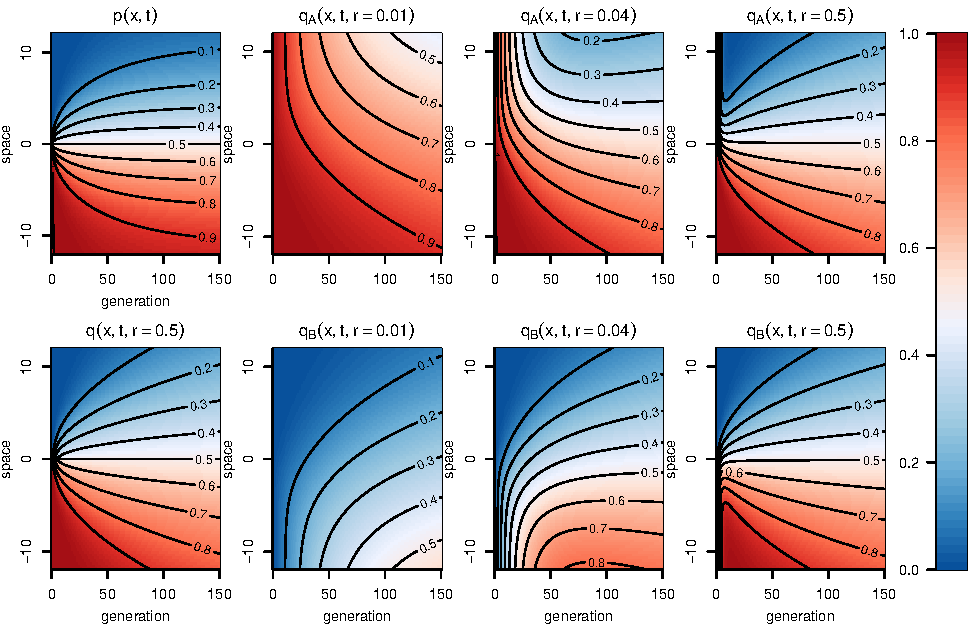
\includegraphics{figs/linked-frequencies.pdf}
    \caption{
        \textbf{Probabilities of $A$ ancestry,}
        across space (vertical axis, in units of $\sigma$) 
        and time (horizontal axis, in generations).
        In each plot, color corresponds to the expected frequency of $A$ ancestry
        at a particular location in time and space.
        The selection coefficient is $s=.02$.
        \textbf{Top left:} at the selected site, showing establishment and stabilization of the cline
        on a time scale of $1/s=50$ generations.
        \textbf{Bottom left:} at an unliked site,
        with cline flattening continuing with $\sqrt{t}$.
        \textbf{Remaining figures} show frequencies of $A$ ancestry \emph{conditional}
        on the ancestry at the selected site,
        at different distances from the selected site ($r=.01$, .04, and 0.5 Morgans),
        as described in the text (see definition of $q_z(x,t,r)$).
        See Figure \ref{sfig:linked_cline_heatmaps_longtime}
        for the same figure over a longer period of time.
    }
    \label{fig:linked_cline_heatmaps}
\end{figure}


\paragraph{Linked clines}
We can use this diffusion model for lineages to find expected clines in ancestry,
i.e., the expected proportion of individuals who inherit from species $A$,
as a function of space, time, and position on the genome.
Precisely, we need the probability that 
an allele sampled $t$ generations after secondary contact at location $x$,
at recombination distance $r$ to a selected allele of type $z$,
is inherited from an individual of ancestry $A$,
where $z$ can be either $A$ or $B$.
We denote this probability $q_z(x,t,r)$.
In the notation above,
\begin{align}
    q_z(x,t,r) = \P^x \{Z_t = A \given X_0 = x, \; Z_0 = z\} .
\end{align}
(Recall that $Z$ depends implicitly on $r$.) \revpoint{1}{7}
The description above implies that $q_z$ solves the following Kolmogorov backward equation:
\begin{align}
    \begin{aligned}  \label{eqn:q_pde}
    \frac{d}{dt} q_A(x,t,r) 
            &= 
                \frac{\sigma^2}{2} \frac{d^2}{dx^2} q_A(x,t,r) 
                + \sigma^2 \frac{d}{dx} \log(p(x,t)) \cdot \frac{d}{dx} q_A(x,t,r) 
            \\ &\qquad {} + 
                r (1-p(x,t))(q_B(x,t,r)-q_A(x,t,r))  \\
        \frac{d}{dt} q_B(x,t,r) 
            &= 
                \frac{\sigma^2}{2} \frac{d^2}{dx^2} q_B(x,t,r)
                + \sigma^2 \frac{d}{dx} \log(1-p(x,t)) \cdot \frac{d}{dx} q_B(x,t,r) 
            \\ &\qquad {} + 
            r p(x,t) (q_A(x,t,r)-q_B(x,t,r))  ,
    \end{aligned} 
\end{align}
with boundary conditions $q_A(x,0,r)=1$ and $q_B(x,0,r)=0$.
% and where $\grad$ is the gradient.
The three terms in these equations come from Brownian movement of a linages 
(i.e., the smoothing action of local dispersal),
the tendency of a lineage to inherit from regions where its type is more common 
(i.e., the net flux induced by reduced fitness in the hybrid zone),
and recombination between selected backgrounds, respectively.
We note that because recombination occurs within a deme, the recombination terms in equation \eqref{eqn:q_pde} are quite standard \citep{HartlClark}. \revpoint{1}{4}
%\alisa{this is fwd-in-time notation. should we change it to bwd-in-time?}
%\plr{This equation should be forwards in time, since it's the Kolmogorov backward equation
%applied to a backwards-time process!}

We will have more use for the differential operators on the right-hand sides of these equations,
so define these as
$
G^A = 
(\sigma^2/2) \frac{d}{dx^2}
+ 
\sigma^2 \frac{d}{dx} \log(p(x,t)) \cdot \frac{d}{dx} 
$
and
$
G^B = 
(\sigma^2/2) \frac{d}{dx^2}
+ 
\sigma^2 \frac{d}{dx} \log(1-p(x,t)) \cdot \frac{d}{dx} 
$
,
so that equation \eqref{eqn:q_pde} can be written more compactly as
\begin{align*}
    \frac{d}{dt} q_A &= G^A q_A + r (1-p) (q_B-q_A) \\
    \frac{d}{dt} q_B &= G^B q_B + r p (q_A-q_B) .
\end{align*}
In technical terms, $G^A$ and $G^B$ are the generators of the diffusions of lineages of selected alleles of ancestry $A$ and $B$, respectively;
informally, they encode the stochastic motion of lineages at the selected loci.


\paragraph{Numerical computation}
To determine how the cline at a linked locus is expected to relax, 
%\alisa{and to confirm the behavior of our model to previously established results,}
%\plr{(got a reference for that?)} 
we can solve the partial differential equations \eqref{eqn:cline_pde} and \eqref{eqn:q_pde} numerically.
For instance, Figure \ref{fig:linked_cline_heatmaps} shows a heatmap of $p(x,t,r)$, 
the expected frequency of ancestry $A$ at location $x$ and time $t$ 
at a site at recombination distance $r$ from the selected site,
which is computed as the frequency of ancestry $A$ on each selected background weighted by the frequencies of each background:
$q(x,t,r) = p(x,t) q_A(x,t,r) + (1-p(x,t)) q_B(x,t,r)$. 
The equations are solved numerically in R, using the ReacTran package \citep{soetaert2012reactive}.

\paragraph{Haplotype lengths}
We now develop our model further to find the frequency at which \emph{entire} blocks of genome (haplotypes) 
of a single ancestry are found, at a given location and time.
Suppose we sample an individual at spatial location $x$ and time $t$ after the initiation of gene flow,
and genotype them on the genomic segment between positions $a$ and $b$, relative to the selected site. 
We are interested in the probability $g_z(x,t;a,b)$ 
of finding an entire segment $(a,b)$ of ancestry $A$ 
given that the individual has selected allele of type $z$.
\revpoint{1}{10}
For instance, $g_B(0,10;0,.2)$ is the probability that an individual carrying a selected $B$ allele sampled at the center of the zone
at $t=10$ has a block of $A$ ancestry for 0.2 Morgans to the right of the selected site.

As in \citet{sedghifar2015spatial}, 
a given block of genome is inherited along a single lineage ever since the most recent recombination event
that fell within that block.
Prior to this, there are two lineages to follow (see Figure~\ref{Fig:schematic}),
and so lineages behave as labeled, branching diffusions,
where the total branching rate is conserved. 
We do not consider subsequent coalescence.
The general description of the process, again looking backwards in time, is as follows:
The lineage of a segment of genome moves as a linked locus described in equations \eqref{eqn:lineage_motion},
with recombination distance $r$ equal to the rate at which the segment recombines away from the selected site.
(If the selected site lies inside the segment, $r=0$.)
Additionally, at rate equal to the genetic length of the segment,
recombination occurs within the segment, at which point it splits in two at a uniformly chosen location between $a$ and $b$,
each of which proceeds as before, independently. 
In this description,
$g_z(x,T;a,b)$ is then the probability that all branches are found on the $A$ side of the hybrid zone
at the time of secondary contact $T$ units of time ago.
We will write $r(a,b)$ for the distance from the segment to the selected site:
always taking $a \le b$,
$r(a,b)=0$ if $a \le 0 \le b$ and $r(a,b)=\min(|a|,|b|)$ otherwise.

The resulting equation is similar to \eqref{eqn:q_pde} with a term added for branching,
which is written (omitting the $(x,t)$ for conciseness):
\begin{align}
    \begin{aligned} \label{eqn:g_pde}
        \frac{d}{dt} g_A(a,b) 
        &= G^A g_A(a,b) + r(a,b) (1-p) (g_A(a,b)-g_B(a,b))
            \\ {} & \qquad 
            + (1-p) \left( 
                \int_a^{\min(0,b)} g_B(a,\theta) g_A(\theta,b) d\theta
                + \int_{\max(0,a)}^b g_A(a,\theta) g_B(\theta,b) d\theta 
            \right)
            \\ {} & \qquad 
            + p \int_a^b {
                g_A(a,\theta) g_A(\theta,b) 
            } d\theta
            - (b-a) g_A(a,b)  ,
    \end{aligned} 
\end{align}
Here the first term ($G^A g_A$) represents spatial mixing,
and the second term results from recombinations \emph{between} the block and the selected site 
in heterozygotes, which switch the identity of the linked, selected locus without splitting the block
(the factor $(1-p)$ is the probability that the block, initially linked to an $A$ allele, encounters a $B$ allele
under the assumption of locally random mating).
In the integrals, $\theta$ is the genomic position of the recombination event.
The third term accounts for such recombinations in a heterozygote: 
the portion of the block nearest the selected site remains linked to an $A$ allele, 
and the remaining portion becomes linked to a $B$ allele 
(e.g., the lower recombination event shown in Fig.~\ref{Fig:schematic}).
To account for cases where the selected locus lies outside the interval [a,b],
we say that the integral $\int_a^{\min(0,b)}$ is zero if  $a>0$ 
and likewise $\int_{\max(0,a)}^b$ is zero if $b<0$.
The last integral results from recombination inside the block in homozygotes for $A$ 
(e.g., the upper recombination event in Fig.~\ref{Fig:schematic}),
and the final term balances the outflux due to all recombinations.
The equation for $g_B(x,t;a,b)$ is identical after exchanging $A \leftrightarrow B$ and
$p \leftrightarrow (1-p)$.
The boundary conditions are $g_A(x,0;a,b)=1$ and $g_B(x,0;a,b)=0$.

\paragraph{Numerical solutions}
Notice that equations \eqref{eqn:g_pde}
are hierarchical in $(a,b)$:
the equation for haplotype identity probabilities on a segment $(a,b)$ depends only on those probabilities for segments contained in $(a,b)$.
This is useful for numerical solutions, %`efficient` may be an overstatement
described in more detail in Appendix \ref{apx:haplotype_calcs}.


\paragraph{Correlations in ancestry}
To compute correlations in local ancestry
(i.e., ``ancestry disequilibrium'', as in \citet{pool2015mosaic,Schumer2016}),
we need only follow lineages at two sites, instead of an entire region. 
Doing so only requires computing correlations in ancestry between markers,
which can be done directly using our numerical code;
see Appendix~\ref{apx:haplotype_calcs} for more detail. \linelabel{ll:ld_comps}


%%%%%%%% %%%%%%%%%%
\subsection*{Simulations}

We implemented forwards-time simulations of a one-dimensional grid of demes
with non-overlapping generations and fixed population sizes (a Wright-Fisher model). Individuals are diploid, with haploid number $n=2$ chromosomes, each of length 1 Morgan. One chromosome pair harbors, at position 0.5M, a single locus that reduces fitness by $s$ in heterozygotes, while the other contains no sites under direct selection.

Each deme has exactly $N_d$ diploid hermaphroditic individuals at the start of each generation.
Then, every individual disperses to a (possibly) new deme
by choosing a Gaussian displacement with mean zero and variance $\sigma^2$,
then dispersing to the nearest deme. \revpoint{AE}{5}
% can migrate to a new deme offset by $\lfloor Z + 1/2 \rfloor$ from their original position,
% where $Z$ is a Gaussian random variable with mean zero and variance $\sigma^2$.
% (Here $\lfloor z \rfloor$ is the largest integer less than or equal to $z$,
% so this equivalently takes a centered Gaussian displacement and assigns it to the nearest deme. 
(The mean displacement is zero, and when comparing to theory we compute $\sigma$ as the standard deviation of this discrete distribution.)
Migrants past either end of the range remain at the terminal demes.
Then, 
fitnesses are computed (heterozygotes at the selected locus have fitness $1-s$; homozygotes have fitness 1),
and in each deme $N_d$ pairs of parents are chosen, with replacement,
with probability proportional to their fitness and selfing allowed.
Since migration is not conservative, demes may have no available parents;
in this case, parents are chosen from other demes with probability proportional to fitness
multiplied by $\exp(-x^2/\sigma^2)$, where $x$ is the distance to the other deme. \revpoint{2}{4}
The next generation is formed by carrying out meiosis in each parent
and combining the resulting gametes such that each pair of parents leaves one descendant.
Meiosis results in alternating blocks of the gamete's chromosome
being inherited from the two parental chromosomes,
with the blocks separated by a Poisson(1) number of uniformly chosen recombination points along the chromosome,
and the order of the parental chromosomes chosen randomly.
The simulation software works by recording, for each chromosome, 
a list of ancestry breakpoints, and the index of the ancestor from which 
the chromosome inherited that genomic region.
We then assigned ancestry at individual loci by looking up which side of the zone the ancestor lived on.

For efficiency, in most simulations the number of demes was only 3--5 times wider than the stable cline width. \linelabel{ll:narrow_sims}
We verified that the size of the simulated region did not affect dynamics in the center of the zone
by running additional simulations on wider regions
(as we did for numerical solutions of PDE);
an example is shown in Figure \ref{sfig:extra_long_cline}.

The simulations were executed in R, with scripts available at
\url{https://github.com/petrelharp/clinal-lineages}.

\begin{figure}
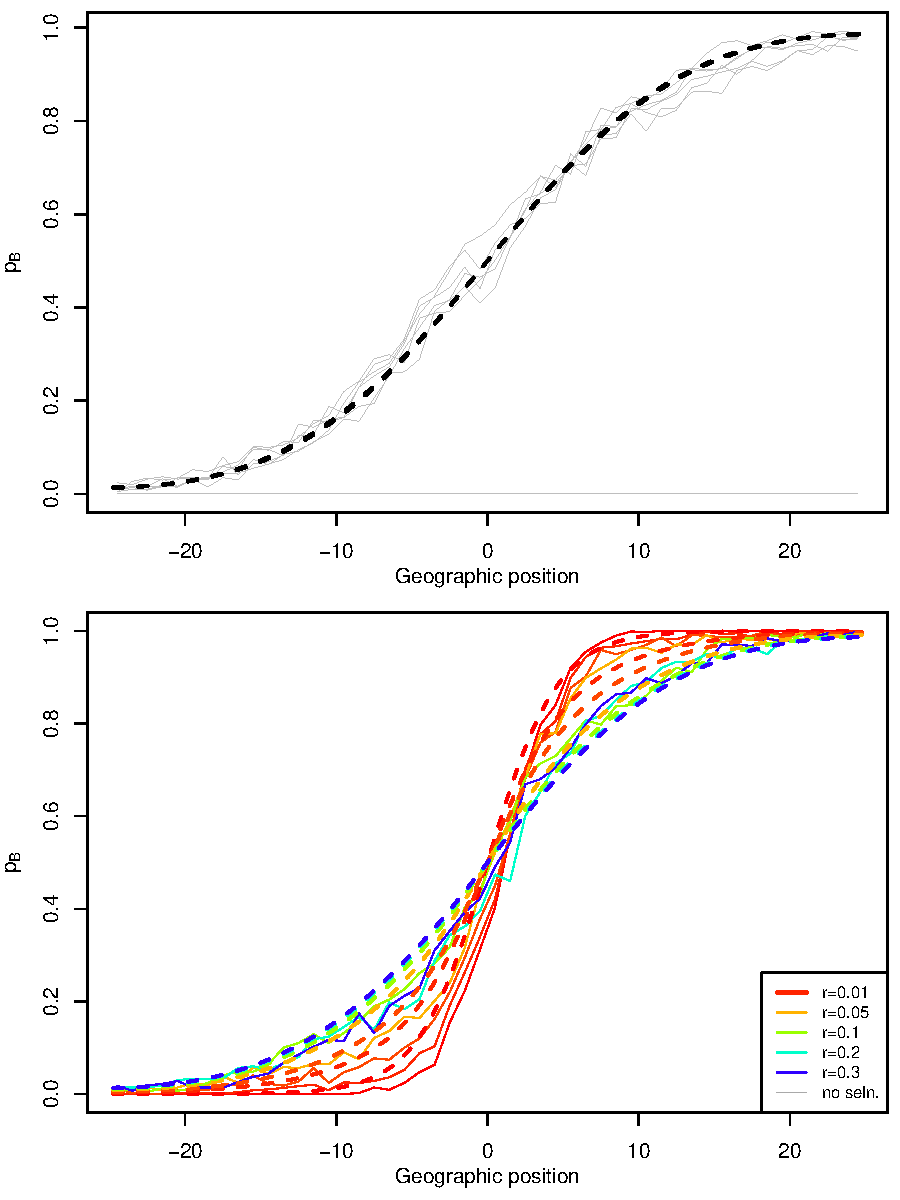
\includegraphics{figs/alleleFrequencies_sim_comparison_revision_original.pdf}
    \caption{
        \textbf{Comparison of simulated to theoretical clines:}
        Frequency of ancestry $B$,
        across geography at different physical positions on the genome, simulated for a hybrid zone
        $T=100$ generations after secondary contact, with $s=0.1$,
        using 50 demes, each with 500 diploid individuals and $\sigma=1$.
        In each figure,
        each line represents a locus some distance $r$ away from the true target of selection, 
        and $r=0$ represents the locus that is under selection. 
        Dotted lines are expected frequencies of $B$ ancestry $1-q(x,t,r)$
        (unconditional on the ancestry of the linked allele), computed numerically.
        \textbf{Top:}
        loci across a chromosome unlinked to the selected locus.
        \textbf{Bottom:}
        loci across the chromosome carrying the selected locus,
        with colors corresponding to different values of $r$, from red (tight linkage to selected site) to blue (distantly linked).
        The two sets of clines are shown superimposed in Figure \ref{alleleFreq_tau100}.
    }\label{fig:alleleFreq_tau100_comparison}
\end{figure}

\subsection*{Measures of introgression}


The above theory and simulations generate predictions about patterns of ancestry surrounding selected loci. 
In reality, however, such loci are not usually known, so it is useful to have per-site statistics that may allow for detection of candidate targets of selection. 
The most straightforward measure is $l_B(m,x)$,  
the mean length of all contiguous segments of ancestry $B$ sampled at position $x$ that contain genomic position $m$.
Likewise, $l_A(m,x)$ is the mean length of segments of ancestry $A$.
We compute similarly the unconditioned mean block length $l(m,x)$
by averaging all segment lengths without regard to ancestral identity.

We also look at the mean length of the two chunks, $m-$ and $m+$, that flank, to the left and right respectively, 
the block of unbroken ancestry containing $m$. 
As described below, these blocks tend to be \emph{shorter} than average when $m$ is the selected site,
motivating us to define the statistic
\begin{align}
     C(m,x) =  \frac{2\sum_i{l_B(m_i,x)}}{\sum_i{l_A(m_i+,x)+l_A(m_i-,x)}}
\end{align}
where $m_i$ is the block length in individual $i$, and the sum is over individuals at location $x$.
The statistic $C$ is the mean block length around $m$ in the population, 
divided by the mean lengths of the two blocks directly flanking the block containing $m$. 

To identify regions of the genome with abnormal distributions of block lengths, 
we compute $l_B(m,x)$ and $C(m,x)$ at a grid of positions across geography and across the genome. 
From these, we compute normalized versions $\bar l_B(m,x)$ and $\bar C(m,x)$
by dividing by the empirical mean across the genome for each geographic location $x$:
for instance, $\bar l_B(m,x) = n_x l_B(m,x)/\sum_i l_B(m_i,x)$,
where the sum is over the $n_x$ individuals at location $x$.
While there is useful information contained in the geographic distribution of block length patterns, 
obtaining good spatial sampling can often be difficult, 
and this allows us to search for patterns if block lengths are only known within relatively few populations. 

We are able to partially trace the genealogy of haplotypes in our simulations. 
In particular, we wish to know the relative number of ancestors from $T$ generations ago that are represented in present day populations at a given locus, given the frequency of a particular ancestry. 
This is a reflection of the average size of a haplotype's family, 
and is potentially a source of additional information about selection. 
Within each deme $x$, we calculated $F_B(m,x)$, which is the number of independent ancestors from time $T$ contributing to the pool of alleles of ancestry $B$ at site $m$, 
divided by the number of individuals of ancestry $B$ at site $m$.


%\subsection*{Data}
%We compare the predictions of our model to genomic data obtained from individuals sampled a naturally occurring hybrid zone between \emph{Mus m. musculus/M. m. domesticus} \cite{Turner2011,Turner2014}. The genomic data generated by \citep{Turner2014} was for a mapping population generated by mating wild-caught individuals. Because some individuals were mated multiple times, the mapping population comprises many closely related individuals. We approximate wild population samples by restricting our analysis to genotyped individuals that had both parents sampled in the same location in such a way that none of the individuals shared a parent (see table for list of individuals). Approximately 280,000 SNPs were represented in the final dataset. 

%Ancestry blocks were estimated using ChromopainterV2 \cite{Lawson2012} and STRUCTUREv2 \cite{Falush2003} with $k=2$.


%Although we expect the age of this hybrid zone to correspond to historical human movement, and therefore be thousands of years old \cite{Teschke2008}, weighted the physical scale of ancestry-disequilibrium (both in the form of weighted ancestry-LD \citep{Loh2013} and ancestral block lengths) suggest relatively recent hybridization. Specifically, the high LD between quite distantly linked SNPs in the FS population suggests that a relatively high proportion of early-generation hybrids, whereas the rapid decay of LD in the the TU population reflects a much older hybridization event. Importance of geographic distribution of popgen patterns. 

%\begin{table}
%\begin{tabular}{l|c|c}
%Individual ID  & Population \citep{Turner2011} & Longitude(E)\\
%\citep{Turner2014}& \citep{Turner2011}&\\
%\hline
%FP112 & FS&11.665\\
%FP67 & FS &11.665\\
%FP114 & FS &11.665\\
%FP79 & FS &11.665\\
%FP152 &  FS &11.665\\
%FP11 & GL &11.965\\
%FP111&GL &11.965\\
%FP59 & HA  &11.721\\
%FP92 & HA &11.721\\
%FP7 &  HA  & 11.721\\
%FP45 & HA&11.721\\
%FP244& HO &11.693\\
%FP9&   RE&11.994\\
%FP5 &  RF&11.767\\
%FP78 &  SO &11.539\\
%FP52 &  SO &11.539\\
%FP180& SO &11.539\\
%FP14 & ST&11.539\\
%FP40 & ST&11.539\\
%FP145 & TU&11.748\\
%FP29&  TU&11.748\\
%FP135& TU&11.748\\
%\end{tabular}
%\end{table}


%%%%%%%%%%%%%%
\section*{Results}


\subsection*{Single locus clines}

As expected, clines in simulations form and begin to flatten, 
with ancestry frequencies at the selected site maintaining a stable shape,
and tightly linked sites flattening more slowly than distant sites.
This is seen in Figure \ref{fig:alleleFreq_tau100_comparison},
and supplementary Figures \ref{alleleFreq_tau100}, \ref{alleleFreq_tau100_weaker_s} and \ref{alleleFreq_tau1000}. 
Clines in ancestry frequency matched expected values found from deterministic theory
up to stochasticity due to genetic drift, which is more pronounced at lower population densities.
For instance, Figure \ref{fig:alleleFreq_tau100_comparison} shows that expected clines computed from equation \eqref{eqn:q_pde}
match simulated clines quite well.
Figures \ref{sfig:condAlleleFreq_tau80_comparison}, \ref{sfig:condAlleleFreq_tau320_comparison}, and \ref{sfig:condAlleleFreq_tau1280_comparison}
show this comparison with a lower population density than in Figure \ref{alleleFreq_tau100},
and separating linked clines based on the identity of the linked selected allele.
The agreement is good over hundreds of generations, \revpoint{2}{6}
although as the clines flatten they are seen to wobble
(which happens at rate proportional to $\sqrt{T}$; \citet{Barton1979a}).
%% \plr{I tried to rephrase this:}
% but by $T=1280$ generations,
% stochasticity has substantially moved allele frequencies range-wide,
% \yb{which is in accordance with previous theory showing that tension zones wobble at a rate proportional to $\sqrt{T}$ \citep{Barton1979a}.}
% %\citep[which is unsurprising, as the total population size is only 5,000 diploids:][]{Polechova2011}.
% \plr{(With effective population size only thousands, once you get to 1,280 generations, it doesn't matter that you're simulating a spatial population;
% drift will kick in and move frequencies \emph{range-wide}.
% We see that in Figure \ref{sfig:condAlleleFreq_tau1280_comparison}.
% That's what I was trying to say here.
% Total population size is not irrelevant.)}

Loci not under direct selection can in principle spread across the cline unimpeded. 
In practice, however, it can take quite some time for even unlinked neutral loci to homogenize,
due to the decreased fitness of heterozygotes \citep{barton1986barrier}
and the relative slowness of diffusive movement.
We display the spread of ancestry across space and time in Figure \ref{fig:linked_cline_heatmaps}. 
The cline in ancestry at a locus $r$ Morgans from the selected site
will have flattened out to distance $x$ (say, on the $B$ side)
if there is a good chance that the corresponding lineage that begins linked to a $B$ allele
traces back to an $A$ allele on the opposite side of the hybrid zone.
Since lineages linked to $B$ alleles move nearly as unbiased Brownian motion on the $B$ side,
this is only possible if Brownian motion has had enough time to travel distance $x$,
i.e., if $T>\sqrt{x}$.
This square-root flattening is seen in Figure \ref{fig:linked_cline_heatmaps}
(and is discussed for environmentally determined clines by \citet{may1975gene}; but see \citet{durrett2007width}). \linelabel{ll:may_citation}
A linked lineage must also spend at least $1/r$ generations in heterozygotes
to have a good chance of recombining,
so clines with $r<1/T$ will still resemble the selected cline,
which can also be seen in Figure \ref{fig:linked_cline_heatmaps}.


In principle, the genomic window about the selected site
in which clines remain narrow could be quite a bit wider,
since the only way to move linked lineages between selected backgrounds is via recombination in a heterozygote,
and heterozygotes for the selected allele are only found at high frequency in the cline.
The majority of lineages are generally pushed away from the cline but have no bias far away,
so the amount of time a lineage spends in heterozygotes should grow as $\sqrt{T}$ for large $T$,
and so the width of the genomic region showing clines about the selected locus could be 
substantially larger than $1/T$. However, this distinction appears hard to observe for realistic parameter values.






%%%%% %%%%%%%%%%
\subsection*{Blocks of ancestry}

The distribution of contiguous ancestry block lengths contains more information than allele frequency alone. 
We are specifically interested in how the tracts of ancestry surrounding the selected locus compares to the rest of the genome. 
Ideal information -- true ancestry assignments for a few simulated individuals sampled from across space -- % YB changed  `raw-data' to information, because ancestry will never be raw-data -- ATGC will
are shown in Figure \ref{Fig:resistanceToIntrogression100g} ($T=100$ generations) and Figure \ref{Fig:resistanceToIntrogression1000g} ($T=1000$ generations).
For the more recent hybrid zone ($T=100$), the selected cline has established,
but linked clines are still flattening.
After a longer period ($T=1000$),
clines over much of the chromosome are flat
(since the width of the entire population is less than $1/\sqrt{T}=31.6\sigma$),
but a distinct enrichment of each ancestry is observed around the selected site.

We expect that, in the absence of selection, blocks of $A$ ancestry across the genome 
will tend to be shorter the further one goes into the $B$ side of the cline,
because they have had more opportunities to recombine with $B$ haplotypes. 
This is seen in Figure \ref{Fig:meanBlockLengthsUnconditioned}.
However, we expect that stretches of $A$ ancestry \emph{containing a selected site} will be longer
than those that do not contain the selected site at the same spatial location,
because lineages containing the selected site have usually been inherited from the $A$ side of the cline recently. 
As discussed above, we expect these lineages move at speed roughly $\sigma\sqrt{s}$,
so (selected) $A$ alleles at distance $x$ from the cline center
have last had an ancestor on the $A$ side of the cline around $x/(\sqrt{s}\sigma)$ generations ago 
(compared to $x^2/\sigma^2$ for a neutral allele).
This implies the scale on which $A$ haplotypes are found surrounding the locus should be no longer than about $\sigma\sqrt{s}/x$.
\revpoint{2}{8}
%\plr{(check predicted decay of mean length $1/x$ in simulations?)}

\paragraph{Identifying selected loci}
The statistics $\bar l(m,x)$ and $C(m,x)$ show promise for identifying selected loci under some circumstances.
As expected, regions surrounding a locus under selection are more resistant to introgression,
as seen in Figures~\ref{Fig:resistanceToIntrogression1000g} and \ref{Fig:resistanceToIntrogression100g}.
When present, we expect haplotypes that contain the locally less common allele
to be longer than the genome-wide average.
Indeed,
as shown in Figures \ref{Fig:blockLengthsZoom}, \ref{Fig:blockLengths} and \ref{Supp:blockLengthHeatmap},
the mean length of such haplotype blocks is up to three times longer
than the average for that geographic location,
peaking quite sharply around the location of the selected site.

Using the fact that genomic regions are inherited from ancestors $T$ generations ago
in blocks of size roughly $1/T$, \revpoint{1}{6}
we can provide some intuition about the physical scale of the expected signal.
There will be a long segment of $A$ ancestry
if many such adjacent blocks are all inherited from the $A$ side.
Ancestries of neighboring blocks are correlated,
due to the branching process described above. 
But, if we assume they are independent, 
then since the block surrounding location $r$ in an individual at geographic location $x$ is of ancestry $A$ with probability $q_A(x,T,r)$,
we'd expect to see, roughly, 
$q_A(x,T,r)(1+2q_A(x,T,r))/(1-q_A(x,T,r))$ 
% P(N=0) = q and if N>0 then is 1 + two independent q-geometrics with mean q/(1-q),
% so is q ( 1 + 2q/(1-q) ) = q(1+2q)/(1-q) .
consecutive blocks of ancestry $A$ about a given site unlinked to the selected site.
(This assumes, crudely, that the number of $A$-blocks on either side of the enclosing block
has a Geometric distribution with parameter $q_A(x,T,r)$.)
This implies the mean length $l(x,r)$ would be $q_A(x,T,r)(1+2q_A(x,T,r))/((1-q_A(x,T,r))T)$,
and the mean conditional length $l_A(x,r)$ would be $(1+2q_A(x,T,r))/(T(1-q_A(x,T,r))$.
Furthermore, we know that if $x=0$ or if $T$ is large and $r$ is not too small, that $q_A$ is close to $1/2$
(so $l_A(x,r) \approx 4/T$);
and for $r<1/T$ that $q_A$ looks like the selected cline.
Also, we know from the discussion above that the lineage of a \emph{selected} $A$ allele,
if it is in the region where $A$ is rare,
moves at speed roughly $\sigma \sqrt{s}$ back towards the $A$ side of the zone,
returning to the region where $A$ is common in about $x/(\sigma \sqrt{s})$ generations.
Therefore, a selected $A$ allele found on the $B$ side of the zone
should carry with it a haplotype of average length $\sigma \sqrt{s}/x$
that looks like haplotypes from the center of the zone.
This analysis suggests that $A$ haplotypes in the center of the zone should be of average length $4/T$;
this is indeed what is seen at distant sites, for instance, in Figure \ref{sfig:blocksAlongChromAncBConditioning_nonnormalized}.
Haplotypes at the selected site are expected to be longer, but still of a length proportional to $1/T$,
suggesting that the normalization in the statistic $C(x,m)$ is appropriate,
as shown in Figure \ref{Supp:adjacentBlocks},
although a numerical prediction of the value of $C(x,m)$ is elusive.
% \alisa{Above argument assumes independence between lineages. Does this make block lengths conservative? }
% PR: yes, maybe, but that correction seems like a small one, and it's not getting very quantitative predictions;
% a more serious issue is that it's ignoring that the next block has a different $r$.


The mean haplotype length found without conditioning on ancestry, $l(x,m)$,
shows a smaller increase near the selected locus, because most blocks will be of the locally common type, and so do not trace back to regions of different block lengths (Figures \ref{Fig:meanBlockLengthsUnconditioned}, \ref{Supp:blockLengthHeatmapNoAnc} and \ref{Supp:blockLengthNoAnc}).

Power will be optimal at intermediate values of $s$.
If selection is too strong, it may be difficult to observe this signal
due to a lack of introgressed selected sites,
while if selection is weak, the selected lineage does not move very fast,
and the hybrid zone is wider, allowing more recombination,
and so the strength of signal from elevated $l_B(m)$ is diminished.
For instance, no signal is seen in Figure~\ref{sfig:blockLengthPlot_t1000_s0.001}.
% Indeed, if $s$ is less than $x/(\sigma T)$, then only one block of ancestry $A$ is expected to be seen about a selected $A$ allele,
% and $l_A(x,m)$ is expected to be $2/T$.
For similar reasons, power and resolution are best at intermediate $T$.

% Additionally, we find that $l_A(m\pm)$, the length of blocks adjacent to blocks containing $m$, are shorter than average when $m$ is in a block of unbroken ancestry surrounding a selected site on the ``wrong side'' of the side of the zone.  (Figure~\ref{Supp:adjacentBlocks}). This pattern provides an avenue for further enhancement of the block-length signal around a selected locus, by measuring $C(m)$  (Figures~\ref{Supp:ratioBlockAdjacent},~\ref{Supp:ratioBlockAdjacentHeatmap}).





\begin{figure}
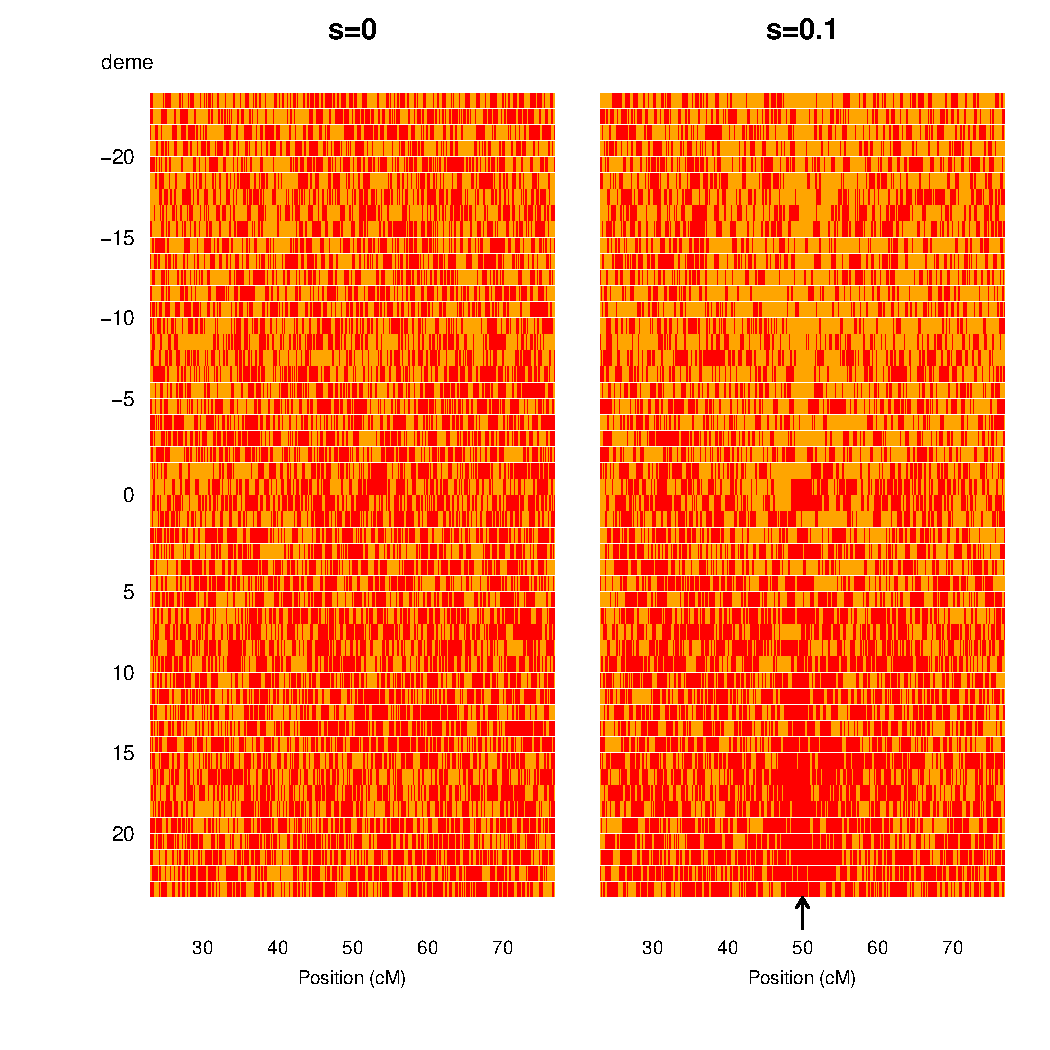
\includegraphics[width=\textwidth]{figs/plot_chromosomes_tau1000_zoomed.pdf}
\caption{
    \textbf{Ancestry blocks for randomly sampled chromosomes} across a hybrid zone of age $T=1000$.  % YB changed from `assignment' to `blocks' because we are interested in the blocks not the assignment of them...
    Here we compare chromosomes of length 1M from a neutral zone to a zone that has a single under-dominant locus with $s=0.1$
    in the middle of the chromosome (indicated by black arrow). 
    Red blocks along the chromosome denote ancestry $B$, and orange blocks are ancestry $A$. 
    The simulation was performed in a population with 50 demes, 
    each with 500 diploids, and $\sigma=1$.
    An analogous figure at $T=100$ is shown in Figure \ref{Fig:resistanceToIntrogression100g}.
}\label{Fig:resistanceToIntrogression1000g}
\end{figure}






\begin{figure}
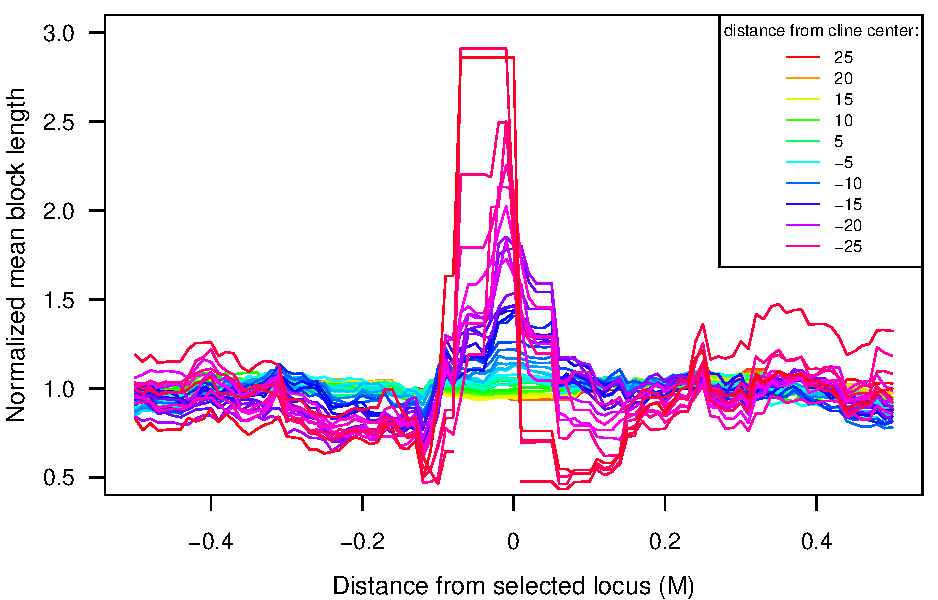
\includegraphics{figs/s0point01_BlocksAlongChromAncBConditioning.pdf}
\caption{\textbf{Normalized mean enclosing block length}, $\bar l_B(m,x)$, along a simulated chromosome of length $1M$ with selected locus of $s=0.01$ at position $0.5M$ in a hybrid zone of $T=1000$. 
    Here each line shows $\bar l_B(m,x)$, in a given deme some distance from the zone center. % , and is normalized by dividing by mean $l_B(m)$ along the chromosome within the deme. 
    Chromosome were sampled across the hybrid zone, which consists of 50 demes, each containing 500 diploid individuals. 
    The same simulation and statistic are shown in Fig.~\ref{Fig:blockLengths}, on coarser genomic scale.
}\label{Fig:blockLengthsZoom}
\end{figure}


%%%%%%
\subsection*{The size of migrant families}

Within-ancestry haplotype diversity, i.e., the number of ancestral haplotypes of each type,
could provide additional information about whether introgression is through relatively few, successful migrants, 
or through many migrants that each contribute relatively little. 
In our simulations, the average local family size of a selected $B$ allele ($F_B(m,x)$) decreases with distance into the $A$ side of the hybrid zone, 
and is lowest far away from the zone center, where ancestry $B$ is at low frequency (Figure~\ref{Fig:family_size}). 
Unlinked loci have local family sizes similar to neutral simulations,
and loci linked to the selected locus have intermediate sizes.
This pattern is consistent with the prediction 
% our theoretical results showing   % sounds pretentious to call the obvious observation 'our results'
that unfit lineages tend to be recent migrants,
which will have smaller families.  

%\alisa{add motivation-- additional information in haplotype diversity. Present alternate hypotheses. This ties in with our world view within our model}
%As expected, we find that the average family size of a $B$ allele decreases with distance into the $A$ side of the hybrid zone. 
% $F_B(m,x)$ is highest on the size of the hybrid zone where individuals of ancestry $B$ predominate. 
%We find that at the selected locus, $F_B(m,x)$ decreases with x, and is lowest far away from the zone center, where ancestry $B$ is at low frequency  (Figure~\ref{Fig:family_size}). As $m$ moves further away from the target of selection, the average family size recovers to expected values under neutrality.
%One interpretation of this observation is that migrants tend to leave few offspring before being removed from the population by selection, leaving behind small families. In conjunction with block length, measuring $F$ can provide an additional signal for characterizing lineages strongly influenced by selection, by looking at levels of haplotype diversity in populations along a hybrid zone.


\begin{figure}
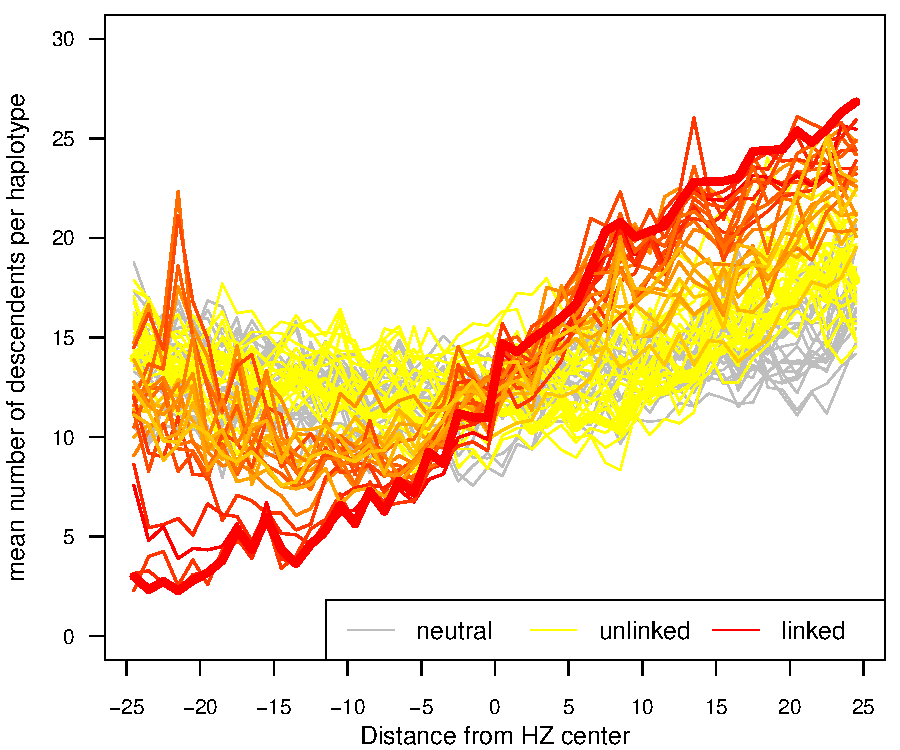
\includegraphics{figs/family_size_tau1000_revision.pdf}
\caption{\textbf{Mean family size of haplotypes.} The number of individuals of ancestry $B$ per number of ancestors ($F_B(m,x)$) from secondary contact occurring $T=1000$ generations ago, represented across geographic space. The hybrid zone is 50 demes, each containing 500 diploid individuals.
 Each red or orange line represents a site some distance away (ranging from 0 - 0.5cM) from the selected site (here $s=0.01$ and $\sigma=1$). Yellow lines are corresponding positions on an unlinked chromosome with no selected loci, and grey lines are corresponding positions in a simulation with no selection.  Bold lines depict the target of selection when present, and corresponding position on chromosomes not harboring any selected sites.}\label{Fig:family_size}
\end{figure}


\section*{Discussion}

Using a combination of theory and simulations, we present a description of the process of cline formation and haplotype structure in a relatively young (i.e., non-equilibrium) hybrid zone. \linelabel{ll:discussion_summary}
We show why clines establish over time $1/s$, 
and why lineages of selected loci tend to move back towards their `ancestral home' when in a geographic region where they are unfit. 
This occurs at speed $\sigma\sqrt{s}$. Based on this we predict, and observe in simulations, that blocks of ancestry surrounding these selected loci are longer, especially when distant from the center of the cline, than those surrounding neutral loci. 
This extends previous theoretical work on hybrid zones, which has primarily focused on stable clines in allele frequency. 
Additionally, our work suggests that the ancestry block length distribution can help detect targets of purifying selection in hybrid zones.  
The resolution of this approach is expected to scale with $1/T$, as this is the physical scale over which linked clines persist.  

\subsection*{Genomic signals associated with targets of selection}

Popular approaches to identifying loci under selection in hybrid zones 
involve identifying alleles that are exceptional in terms of frequency across space, or genome-wide admixture proportion \citep{Porter1997,Gompert2012}.  
The availability of genomic data has made it possible to use local ancestry as an additional source of information. 
In particular, ancestry deconvolution facilitated by programs such as  hapMIX \citep{Price2009}, LAMP \citep{Sankararaman2008} and fineSTRUCTURE \citep{Lawson2012} 
can inform the demographic history of hybridization/admixture from present day samples \citep[e.g.,][]{Hellenthal2014}. 
We described how selection against hybrid incompatibilities  
results in long contiguous blocks of ancestry around these loci. 
This is because regions surrounding selected loci do not readily introgress, 
and so introgressed alleles have been inherited from ``their'' side of the zone recently. %removed `more and less bc we are not comparing anything in this sentence'
We get quantitative understanding from the fact that lineages of
loci under selection move as Brownian motion pushed at speed $\sigma \sqrt{s}$ towards its ancestral side.
In other words, disadvantageous alleles that have encroached deep into the other side of the hybrid zone have done so by chance and, since they do not persist for long on the ``wrong'' side, are likely to have done so relatively recently. Haplotypes surrounding the selected locus therefore have had relatively few opportunities for recombination with different ancestries and this is reflected in longer blocks of contiguous ancestry.

Through our simulations we find also that blocks of ancestry that have crossed the hybrid zone and are closely linked to the selected site without overlapping it (i.e., blocks that are adjacent to the block containing the selected site) are shorter than average for the spatial location (Figure~\ref{Supp:adjacentBlocks}). 
An intuitive explanation for this pattern is that loci physically linked to a selected site have recently come from the center of the zone or beyond. 
Compared to other chromosomes in their new geographic location, these migrants will have on average longer $B$ haplotypes at the selected locus, and shorter $A$ haplotypes nearby. 

Our results suggest that the statistic $l(x,m)$ 
-- the mean genetic length of ancestry surrounding a site of a given lineage --
could help identify selected loci in hybrid zones. 
The ratio of mean adjacent block lengths, $C(x,m)$, alsot shows a very sharp peak at the selected site,
suggesting that, despite the fact that haplotypes surrounding incompatibilities might be quite long, 
genome scans may have the power to extract fine-grained regions near selected loci from the large chunks of ancestry that will often flank these regions. 

Our results focus on the length distribution of ancestry blocks --- a statistic that can only be obtained in the few systems for which dense genetic markers and phase information is known. 
However, as the cost of sequencing continues to drop and long-phased reads become more common, the patterns described here could further aid in the identification of selected sites in hybrid zones in many non-model taxa. 
In the meantime, patterns of elevated pairwise LD, which is easily computed from readily available low-density and unphased genomic data, could offer an alternative path forward for empirical work. 
Importantly, the numerical solutions derived above readily and efficiently predict correlations in ancestry, and so our results can be applied immediately to genotype data for any taxa with markers placed on a genetic map.

Ancestry assignments have the additional benefit that relatively unbiased estimates are possible even with markers of problematic ascertainment
such as those on SNP arrays.
The power and resolution of these approaches depends strongly on the strength of selection,
the time since secondary contact,
and the strength of genetic drift:
in our simulations,
we found good power and resolution at $s=.01$, $T=1000$ generations after secondary contact,
and with hundreds of individuals per dispersal distance.



\subsection*{Assumptions}

Here we review the assumptions we made and their likely impact.

\paragraph{The nature of selection}
Although our assumed scenario of selection against heterozygotes at a single locus is uncommon in nature, 
theoretical and simulation studies show that clines formed by underdominant selection and extrinsic selection 
are effectively indistinguishable without additional information \citep{may1975gene,Barton1993,Kruuk1999}, 
especially over short time scales \citep{Barton1979a},
and their shape is determined mostly by the mean fitness of the heterozygote \citep{Slatkin1973}. 
\revpoint{1}{1}

Our assumption of a single selected locus may have greater consequences. Our model is most relevant to scenarios with few targets of selection scattered throughout the genome, and therefore, our predictions may differ significantly from situations in which the density of selected sites is higher. 
Having numerous selected sites within one ancestry block increases the strength of selection \citep{barton1986barrier}, 
and the relatively short map distances between linked incompatibilities generates a longer unit which is not readily broken up by recombination \citep{barton1986effects}. 
Both factors are expected to result in regions that are surrounded by even longer segments of unbroken ancestry, 
and will impact expectations of genome-wide pattens of clines and block lengths, as well as the resolution to which one could detect targets of selection \citep{Slatkin1975b,Barton1983}. 

To speed calculations and simulations, we assumed a homogeneous, one-dimensional geographical range.
Our analytical results further assumed a large population density, 
effectively working with a deterministic model that ignores coalescence and associated stochasticity.
In contrast, our simulations model regularly spaced demes of finite size.
In reality, populations may be patchily connected, especially at the edges of species ranges where hybrid zones may occur. 
The degree to which inhomogeneous geography would affect the predictions depends on how patchy the zone is;
the differential equations provide a way to evaluate this in specific circumstances.

%It is particularly unfortunate 
%that our analytic calculations do not capture stochasticity arising from coalescence/pedigree structure. 
Extending our analytical results to capture stochasticity arising from coalescence/pedigree structure represents an important future direction.  
Indeed, correlated fluctuations visible in simulations (e.g., Figure \ref{Fig:blockLengths})
are likely due to coupling due to demographic stochasticity;
and simulations at lower density show larger fluctuations than those at higher density.
Furthermore, ignoring pedigree structure can result in an underestimate of covariance in ancestry, as we have ignored additional sharing of ancestry through shared genealogy \citep{liang2014lengths};
but there is nonetheless good agreement between analytic predictions and simulations (which include an explicit pedigree structure).
% suggests that this assumption does not have a severe impact on our major results when population densities are moderately high.



\subsection*{Theory and simulation}
We have taken two complementary approaches,
using both simulation and theory, and comparing the two.
As usual, simulations make fewer biological simplifications,
while theory provides more generalizable conclusions.
To do this, we have described the branching diffusion process that approximates
the lineages along which haplotypes are inherited.
Since the expected motion of a lineage depends on the local frequencies of the selected alleles,
these diffusions are time-inhomogeneous.

The diffusion model for lineages predicts that quantities of interest solve sets of coupled partial differential equations (PDE),
which we have written down.
As there are no known analytical solutions to these PDE,
we have constructed numerical solutions (and provide the source code for doing this).
A main role of these solutions in our work has been to verify that theory based on the diffusion model of lineages
matches realistic, individual-based models.  \revpoint{AE}{8}
These solutions easily and quickly provide predictions of joint frequencies at small numbers of loci:
about 1 second to compute predicted clines, as opposed to hours for the full simulation.
However, due to the high dimensionality of the haplotype problem (spatial position $\times$ time $\times$ endpoints of the haplotype),
numerical solutions for mean haplotype lengths along the genome can be as computationally intensive as simulations
(although are substantially less noisy).
More work could be done to develop more efficient methods of solution, 
but it may be better to perform more biologically realistic forwards-time simulations that includes coalescence and drift to better characterize the block length distribution.
If however the correlation in ancestry, rather than the block-length distribution, is of interest the PDE approach may be preferable because it is easily modified to provide predictions for spatial and temporally inhomogeneous systems -- for instance, across maps of real landscapes.

%, and is an example of the more general idea of duality for particle systems \alisa{I think this may be beyond the average ME reader?}. 
%\plr{Tracking lineages is duality, has nothing to do with 1D, though.}
%However, this assumes a large population density limit that excludes \plr{coalescence} and makes linages Markov \alisa{not sure about what point this is making? Is there a better way to state this for our intended audience?}.  
%\plr{It means we're ignoring drift/coalescence, an important source of stochasticity; but that's the next paragraph too}
%In contrast, our simulations model regularly spaced demes. In reality, populations may be patchily connected, especially at the edges of species ranges where hybrid zones may occur. While we still believe that the genomic signature of long ancestry chunks around selected sites will still hold in these situations, the strength of this expectation is unclear.

%Lastly, the analytic model presented here lacks \yb{both coalescence and a true pedigree structure}. \alisa{This can result in an underestimate of covariance in ancestry, as we have ignored sharing through genealogy \cite{liang2014lengths}.} 
%The broad agreement between our analytic predictions and simulations that include an explicit pedigree structure suggests that this assumption does not have a severe qualitative impact on our major results, especially for all but the most recently formed hybrid zones.

%Foremost, we have assumed that selection acts against heterozygotes, and that there is a single underdominant locus. This situation is uncommon in nature, since underdominant loci cannot invade when rare, and thus this assumption is likely rarely met. \alisa{We believe, however, that this assumption is unlikely to drastically influence our results, and previous results demonstrating that underdominant loci share similar properties as more realistic genetic models such as ecological selection, mean that our findings here are somewhat generalizable} \citep{Barton1989, Barton1993}



%\plr{(long blocks adjacent to short ones: combine with bit on long blocks)}
%In addition to our finding that ancestry surrounding selected sites is relatively long, our simulations revealed a consistent and unexpected finding. We found, on a given side of the hybrid zone, a transition from the locally adaptive ancestry at the selected site to the alternative ancestry at a closely linked site was short-lived (Figure~\ref{Supp:adjacentBlocks}). Put differently, blocks of `wrong' ancestry that do not overlap the selected site but are closely linked are exceptionally short. A simple intuitive explanation for this pattern suggests itself - loci physically linked to the selected sites can only survive on the wrong side of the hybrid zone for a reasonable amount of time if they recombine away from their ancestry at the locally adaptive site. Because it is then tightly linked to the alternate ancestry at the selected site, this ancestry chunk will largely recombine with the alternate ancestry, and therefore decay rapidly. \yb{This finding suggests that, despite the fact that haplotypes surrounding incompatibilities might be quite long, genome scans may have the power to extract fine-grained regions near selected loci from the large chunks of ancestry that will often flank these regions.}






%One major assumption of our model is that selection acts against heterozygotes -- i.e., that loci are underdominant. 
%Under dominance is quite rare in nature, because underdominant loci cannot invade when rare, and thus our major assumption is likely rarely met. 
%We believe, however, that this assumption is unlikely to drastically influence our results --- previous research has found that under dominant loci  have similar properties in hybrid zones as more realistic genetic models, such as ecological selection \yb{(CITE: (BARTON and HEWITT 1989; BARTON and GALE 1993)}. 
%An additional assumption of our analytical model is that we ignore coalescence.  
%The broad agreement between our analytical and theoretical results suggests that this assumption will also have negligible effect on our results. 

%Also, parent-offspring dispersal is not the same thing as successful-offspring-parent dispersal.


%\alisa{epistasis}
%\alisa{selection here is STRONG, not sure how well this will work on systems in which selection on any given locus is small (most systems)}


\subsection*{Patterns of divergence}  
A number of studies have described heterogeneous patterns of genetic divergence across the genome. 
Work on these ``islands of divergence'' \citep{turner2005genomic,Nosil2009} and related patterns have been largely descriptive \citep{Cruickshank2014,Noor2009}.
Our study here contributes to a model-based understanding of 
how migration and selection may influence such patterns across the genome of hybridizing populations. 
Overall, focusing on lengths of ancestry blocks across the genome brings focus to the processes of migration and selection 
rather than high-level summaries that are somewhat abstracted from the evolutionary process. 



%\plr{seems like a nice point but should be more positive and less snarky.  "Thanks to studies like these, it is time to start explicit modeling, as we have done here..."}
%The past years have witnessed evocative metaphors of seascapes to describe heterogeneous patterns of genetic divergence across the genome.  
%The metaphors of ``islands'', ``continents'' and ``archipelagoes'' of divergence \citep{turner2005genomic, Nosil2009} have inspired much research (and controversy  \citep{Noor2009,Cruickshank2014}) in speciation genomics, but have been largely descriptive.  
%REFS  http://www.ncbi.nlm.nih.gov/pubmed/16076241 http://www.ncbi.nlm.nih.gov/pubmed/19143936 http://www.ncbi.nlm.nih.gov/pmc/articles/PMC2809014/ http://onlinelibrary.wiley.com/doi/10.1111/mec.12796/abstract
%We hope that our work provides a path towards thinking about the process of heterogeneous divergence more concretely. % in terms of the processes of migration, and selection influencing patterns of ancestry across the genome of hybridizing populations.


\subsection*{Adaptive introgression}
%\plr{don't have to call it the hybrid filter, and it looks like maybe I made up that term, but after reading this paper: \citet{martinsen2001hybrid}; these sorts of things are discussed in \citet{barton1986barrier}}

While our focus has been on hybrid incompatibilities, 
unconditionally adaptive loci are expected to easily introgress across hybrid zones \citep{barton1979gene,barton1986barrier,martinsen2001hybrid,arnold2004transfer}. 
Future work could take a similar approach to understand how positive selection shapes ancestry block lengths, and predict  signatures of adaptive introgression in hybridizing populations using similar statistics presented here. These could eventually be combined to gain a fuller understanding of the forces shaping patterns of introgression in hybrid zones. 
In particular, beneficial alleles tightly linked to incompatibilities
cannot introgress until recombination separates them;
our model \alisa{provides some rough expectation on how quickly this should happen}. 

%The best characterized example of adaptive introgression comes from the vitamin K epoxide reductase subcomponent 1 (vkorc1), which seems to have spread from Algerian mice \emph{Mus spretus} to house mice \emph{Mus musculus} from because it confers resistance to the anticoagulant rodenticide, warfarin. \citep{Song2011}. 
%Future work could dress expected genomic signatures of adaptive introgression in hybridizing populations using the number and length of haplotypes of non-native ancestry. 
%Doing so requires an understanding of how positive selection shapes ancestry block lengths in these cases. 

\section*{Acknowledgements}
We thank Graham Coop, Nancy Chen, Emily Josephs, Kristin Lee, Nick Barton and two anonymous reviewers for helpful feedback and suggestions.
PR was supported in part by NSF grant DBI-1262645 and a Sloan Research Fellowship.
\alisa{More info here}

\bibliographystyle{molecularEcology}
\bibliography{library,references}

\section*{Data Accessibility}

All scripts used in production of this paper are available at 
\url{https://github.com/petrelharp/clinal-lineages}
under the GPLv3 software license

\appendix
\setcounter{table}{0}
\renewcommand{\thetable}{S\arabic{table}}
\setcounter{figure}{0}
\renewcommand{\thefigure}{S\arabic{figure}}


\section{Rescaling a discrete model to obtain the lineage motion}
\label{apx:lineage_derivation}

For concreteness, here we describe a discrete model that rescales to the continuous model we consider.

In this discrete model, the total number of individuals at location $x$ is $N(x)$,
and we count ``individuals'' as \emph{haploid},
so each individual is of type either A or B at the selected locus,
and the proportion of individuals of type A and location $x$ and time $t$ is $p(x,t)$
(but, we often neglect the $t$).
Suppose that type A individuals at location $x$ reproduce at rate $s_A(x)$, 
and likewise type B at rate $s_B(x)$.
Assuming locally random mating, we will then have that
$s_A(x) = 1 - s (1-p(x))$ and $s_B(x) = 1 - s p(x)$.

At reproduction, individuals recombine with others in the same location,
with recombination occuring between the locus we follow and the selected locus with probability $r$,
and the offspring choose a new location $y$ with probability $m(x,y)$.
The population dynamics are random, 
but suppose that $N(x)$ is sufficiently large that these do not vary substantially with time.
Suppose this is a Moran model.
There are four things that can happen:
\begin{enumerate}
    \item[$x\xrightarrow{AA}y$] One type A individual at location $x$ reproduces, 
        either does not recombine or recombines with another type A,
        and sends the offspring to $y$.
    \item[$x\xrightarrow{AB}y$] An individual at location $x$ reproduces, 
        recombines with the other type,
        and sends to $y$ an offspring
        who inherits at the selected locus from the type $B$ parent 
        and the at the neutral locus from the type A parent.
    \item[$x\xrightarrow{BA}y$] An individual at location $x$ reproduces, 
        recombines with the other type,
        and sends to $y$ an offspring
        who inherits at the selected locus from the type A parent 
        and the at the neutral locus from the type $B$ parent.
    \item[$x\xrightarrow{BB}y$] One type $B$ individual at location $x$ reproduces, 
        either does not recombine or recombines with another type $B$,
        and sends the offspring to $y$.
\end{enumerate}
These four things happen at rates:
\begin{align}
    & x\xrightarrow{AA}y & \qquad w_{AA}(x,y) &= p(x) s_A(x) \left(1 - r (1-p(x)) \right)  N(x) m(x,y) \\
    & x\xrightarrow{AB}y & \qquad w_{AB}(x,y) &= r p(x) (1-p(x)) \frac{s_A(x)+s_B(x)}{2} N(x) m(x,y) \\
    & x\xrightarrow{BA}y & \qquad w_{BA}(x,y) &= r p(x) (1-p(x)) \frac{s_A(x)+s_B(x)}{2} N(x) m(x,y) \\
    & x\xrightarrow{BB}y & \qquad w_{BB}(x,y) &= (1-p(x)) s_B(x) \left(1 - r p(x) \right) N(x) m(x,y) 
\end{align}
For instance,  \revpoint{2}{10}
there are $p(x) N(x)$ type $A$ individuals at $x$, that reproduce at rate $s_A(x)$;
the chance that each reproduction is with a type $B$ is $(1-p(x))$, 
and the chance there is a recombination that gives the offspring genotype $AB$ is $r/2$;
the offspring has probability $m(x,y)$ to disperse to $y$;
the total rate at which individuals at $x$ with the $A$ allele produce offspring at $y$ with the $B$ allele is the product of these terms,
$p(x) N(x) s_A(x) (1-p(x)) r / 2$.
The second and third rates (for $x\xrightarrow{AB}y$ and $x\xrightarrow{BA}y$) are the same;
they are this value plus the corresponding term
for individuals carrying the $B$ allele producing offspring that carry the $A$ allele.

Note that at equilibrium, we require $N$ to solve
\begin{align*}
  0 = \sum_y N(y) m(y,x) \left\{ p(y)s_A(y)(1-p(x)) - (1-p(y))s_B(y)p(x) \right\} .
\end{align*}

\subsection*{Lineage movement}

These rates tell us the rates at which a lineage will move, backwards in time.
For instance, the rate at which a lineage at the selected locus
currently in a type A individual at location $x$
jumps to another type A individual at location $y$ is equal to the rate of influx of migrants from $y$
divided by the number of A alleles at $x$,
or
\begin{align*}
  r_A(x,y) &= \frac{w_{AA}(y,x)}{p(x)N(x)} \\
  &= N(y) p(y) s_A(y) m(y,x) \frac{ 1 }{ N(x) p(x) } .
\end{align*}

Let $X_t$ denote the position of the lineage of a selected locus of time $A$ at time $t$ in the past,
and let $f$ be test function with $f(\rho)=0$.
Then,
\begin{align}
    \deriv{t} \E[f(X_t) \given X_0=x ] &= \sum_y r_{A}(y,x) ( f(y)-f(x) ) \\
    &= \frac{1}{N(x)p(x)} \sum_y  N(y) p(y) s_A(y) m(y,x) ( f(y) - f(x)  ) . \label{eqn:discrete_generator}
\end{align}


\subsection*{Diffusion limit}
% from notes/lineage-movement.tex

Now suppose that $m(x,y)$ is symmetric, and depends on a parameter $\sigma$ so that as $\sigma \to 0$,
the associated random walk converges to Brownian motion, so that for an arbitrary smooth function $f$,
\begin{align*}
    \lim_{\sigma \to 0} \sum_y \frac{ m(x,y) ( f(y) - f(x) ) }{\sigma^2} = \frac{1}{2} \dderiv{x} f(x) .
\end{align*}
Write $f'(x) = \deriv{x}f(x)$, and note that
\begin{align*}
    \frac{1}{\sigma^2} \sum_y g(y) m(y,x) (f(y)-f(x)) 
    &= \frac{1}{\sigma^2} \sum_y m(y,x) \left( g(y) f(y) - g(x) f(x) + (g(x)-g(y)) f(x) \right) \\
    &= \frac{1}{\sigma^2} \sum_y m(y,x) \left( g(y) f(y) - g(x) f(x) \right) \\
    & \qquad - f(x) \frac{1}{\sigma^2} \sum_y m(y,x) (g(y)-g(x)) \\
    &\xrightarrow{\sigma \to 0} \frac{1}{2} \dderiv{x}\left( g(x)f(x) \right) - \frac{1}{2} f(x) \dderiv{x} g(x) \\
    &= \frac{1}{2} \left( g(x) f'(x) + 2 g'(x) f'(x) + f(x) g''(x) - f(x) g''(x) \right) ,
\end{align*}
which tells us the differential operator that best approximates the discrete sum:
\begin{align}
    \frac{1}{\sigma^2} \sum_y g(y) m(y,x) (f(y)-f(x)) 
    &\xrightarrow{\sigma \to 0} \frac{1}{2} g(x) f''(x) + g'(x) f'(x) . \label{eqn:deriv_limit}
\end{align}

Under these assumptions, combining \eqref{eqn:discrete_generator} and \eqref{eqn:deriv_limit},
\begin{align*}
    \deriv{t} \E[f(X_{t/\sigma^2}) \given X_0=x ] &\xrightarrow{\sigma \to 0} 
    \frac{1}{2} s_A(x) \dderiv{x} f(x) 
    + \frac{1}{N(x)p(x)} \deriv{x} \left\{ N(x)p(x) s_A(x) \right\}  \deriv{x} f(x) \\
    &= \frac{1}{2} s_A(x) f''(x) + \left( s_A'(x) + \log(N(x)p(x))' s_A(x) \right) f'(x) ,
\end{align*}
i.e.\ $X_{t/\sigma^2}$ converges to a diffusion with mean displacement
(``drift'' in diffusion terminology) $\frac{1}{ N(x)p(x)} \deriv{x} ( N(x) p(x) s_A(x) )$ and killed at rate $\rho k(x)$.

In our case, since $s_A(x) = 1 - s (1-p(x))$, the drift is $p'(x)/p(x)$ to first order in $s$;
the time scaling by $\sigma^2$ implies that the Brownian noise and the mean displacement
should both be scaled by $\sigma^2$.


%%%%%%% %%%%%%%%%%%%%
\section{Numerical calculation of haplotype probabilities}
\label{apx:haplotype_calcs}

In this section, we give details for how we found numerical solutions
to the partial differential equations (PDE) of the text,
which are all of reaction-diffusion type.
The R code, with worked examples, is available in our git repository.
Spatial grids were usually chosen to have at least four grid sites per dispersal distance,
but using substantially finer grids did not affect the results.

The forwards-time evolution of the selected alleles,
equation \eqref{eqn:cline_pde}, presents no difficulty;
we use the ReacTran package \citep{soetaert2012reactive} to compute discrete approximations to the diffusion term,
and the deSolve package \citep{soetaert2010solving} to solve the equation.

The equations \eqref{eqn:q_pde} describing probabilities that a lineage descends from $A$ ancestry,
conditional on the linked selected allele, required some more attention.
First, $s>0.1$ the system of equations can be \emph{stiff} 
(as is commonly observed for reaction-diffusion equations),
and hence slow to solve,
because of the extremely steep slope of the selected allele frequency $p(x,t)$.
In practice we used $s<0.1$.
Second, the ReacTran function tran.1D that converts the diffusion portion of the PDE into a system of ODE
contains a term like 
\begin{align*}
    \frac{1}{A(x)} \frac{d}{dx} A(x) f(x) = \frac{d}{dx} f(x) + f(x) \frac{d}{dx} \log A(x) ,
\end{align*}
where $A(x)$ is the interface area between grid cells, and $f(x)$ is the flux.
(See \citet{soetaert2012reactive} for more details.)
Discrete approximations of the left-hand side, as implemented in ReacTran, 
run into numerical difficulties if $A(x)$ is small,
and in our case, $A(x)$ is equal to $p$, the local frequency of the selected $A$ allele.
To avoid this, we made minor modifications to the tran.1D to provide a discrete approximation to the right-hand side.

Haplotype probabilities are obtained from equations \eqref{eqn:g_pde},
which is a coupled system of integro-differential equations in three variables plus time.
One method for solution would be via a Wild sum over the number of recombination events, 
as we did in \citet{sedghifar2015spatial}.
Here, we solved the equations numerically,
again discretizing the equations and using the ode.1D function of the deSolve package.
The reaction-diffusion part is the same as for equations \eqref{eqn:q_pde}.
The functions $g_A(x,t;a,b)$ and $g_B(x,t;a,b)$ are functions of space ($x$), time ($t$), 
and the endpoints of the block in question ($a$ and $b$, with $a<b$).
The second integral in \eqref{eqn:g_pde} is
\begin{align} \label{eqn:unifprod}
    \int_a^b { g_A(a,\theta) g_A(\theta,b) } d\theta .
\end{align}
Conceptually, this is an integral transformation
$g(a,b) \mapsto \int_a^b g(a,\theta) g(\theta,b) d\theta$;
the reason it appears here is that for the entire segment $(a,b)$ to be of ancestry $A$,
if there was a recombination at $\theta$,
the two segments $(a,\theta)$ and $(\theta,b)$ must both be of ancestry $A$
(and, ignoring coalescence, these probabilities are independent).
Suppose we have divided the segment of chromosome into a regular grid, say, $r_1 < \ldots < r_n$.
The natural discretization approximates this transformation by a sum,
and is equivalent to keeping track of only a finite number of loci.
Writing $g_A(i,j)$ for $g_A(x,t;r_i,r_j)$,
the discrete transformation we use corresponding to \eqref{eqn:unifprod}
is $g_A(i,j) \mapsto {}$ the sum
\begin{align*}
    \sum_{k=i}^{j-1} (r_{k+1}-r_k) g_A(i,k) g_A(k+1,j) .
\end{align*}
This is the correct term for the process only tracking loci on the grid, because
for all the alleles at $r_i, r_{i+1}, \ldots, r_j$ to be of ancestry $A$,
when a recombination occurrs between $r_k$ and $r_{k+1}$,
the sequences of alleles at $r_i, \ldots, r_{k}$ and at $r_{k+1}, \ldots, r_j$ must each be of ancestry $A$.
The first integral term in \eqref{eqn:g_pde} is
\begin{align} \label{eqn:biprod}
    \int_a^0 g_B(a,\theta) g_A(\theta,b) d\theta
    + \int_0^b g_A(a,\theta) g_B(\theta,b) d\theta 
\end{align}
We now require that one of the grid points along the chromosome is exactly at the selected site;
say this is $r_\ell = 0$.
The discrete term corresponding to \eqref{eqn:biprod} is
\begin{align*}
    \sum_{k=i}^{\ell-1} (r_{k+1}-r_k) g_B(i,k) g_A(k+1,j) +
    \sum_{k=\ell}^{j-1} (r_{k+1}-r_k) g_A(i,k) g_B(k+1,j) .
\end{align*}
Since these are not easily vectorizable in R, for efficiency
we implemented the discrete transformations in C, using the Rcpp package \citep{Eddelbuettel2011}.
In implementing these,
we kept track of $g_A(i,j)$ in a vector in the order that the upper triangular elements of a matrix are encountered
when traversing the matrix column-wise,
allowing for efficient computation of the sum.

\paragraph{A note on symmetry:}
The equations we present have the symmetry that they are invariant after exchanging $A$ and $B$ and reversing space.
For instance, $q_A(x,t,r) = 1 - q_B(-x,t,r)$.
Using this fact would speed up the code by a factor of two,
at the cost of generality:
as written, it would be easy to modify the code to allow space to be inhomogeneous 
(which would break this symmetry).


%% supplement
\section{Supplementary Figures}
% \documentclass[12pt,titlepage]{article}
% 
% %% THE USEPACKAGES NECESSARY FOR THIS EXAMPLE
% %% NOTE THAT genetics_manu_style MUST BE CALLED AFTER mychicago
% \usepackage{graphicx}
% %\usepackage{figcaps}
% \usepackage[nomarkers,notablist,nofiglist,tablesfirst]{endfloat}
% \usepackage{amsfonts}
% \usepackage{sectsty}
% %\usepackage{subfigure}
% %\usepackage{subcaption}
% \usepackage{natbib} \bibpunct{(}{)}{;}{author-year}{}{,} 
% \usepackage[usenames,dvipsnames,svgnames,table]{xcolor}
% %\allsectionsfont{\sffamily}
% %% THE MANUSCRIPT TITLE
% 
% \usepackage{caption}
% \usepackage[labelformat=simple]{subcaption}
% 
% \usepackage{bibentry}
% 
% \usepackage{xr}
% \externaldocument{hybrid_zone}
% 
% \newcommand{\alisa}[1]{{\em \color{red} #1}}
% \newcommand{\plr}[1]{{\em \color{blue} #1}}
% \newcommand{\yb}[1]{{\em \color{magenta} #1}}
% 
% 
% \newcommand{\given}{\,\vert\,}
% \newcommand{\st}{\,\colon\,}
% \renewcommand{\and}{\,\&\,}
% 
% 
% \begin{document}
\setcounter{table}{0}
\renewcommand{\thetable}{S\arabic{table}}
\setcounter{figure}{0}
\renewcommand{\thefigure}{S\arabic{figure}}
\clearpage
\begin{figure}
    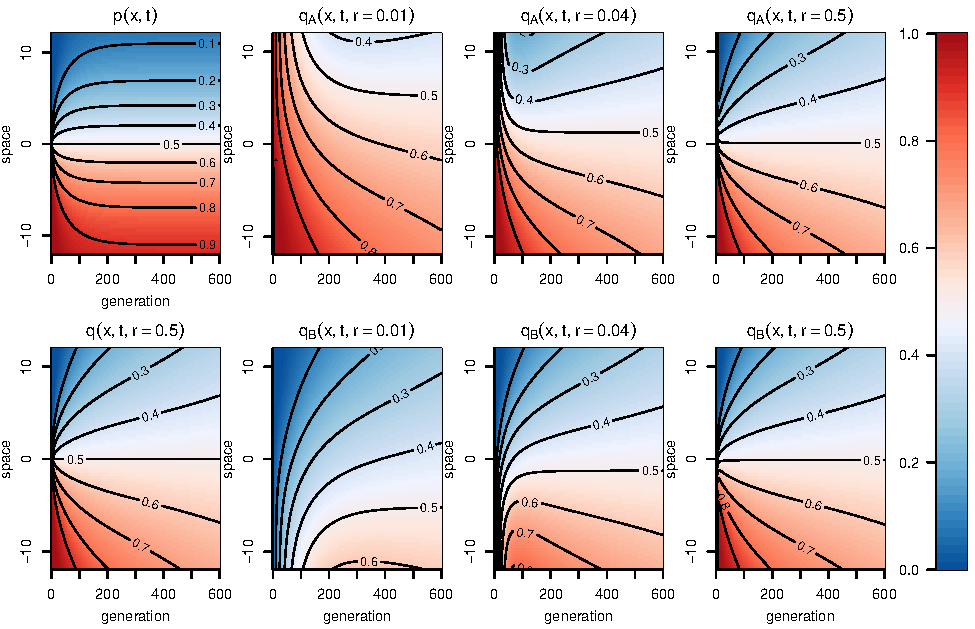
\includegraphics{figs/linked-frequencies-longtime.pdf}
    \caption{
        \textbf{Probabilities of $A$ ancestry,}
        across space (vertical axis, in units of $\sigma$) 
        and time (horizontal axis, in generations).
        In each plot, color corresponds to the expected frequency of $A$ ancestry
        at a particular location in time and space.
        The selection coefficient is $s=.02$.
        \textbf{Top left:} at the selected site, showing establishment and stabilization of the cline
        on a time scale of $1/s=50$ generations.
        \textbf{Bottom left:} at an unliked site,
        with cline flattening continuing with $\sqrt{t}$.
        Remaining figures show frequencies of $A$ ancestry \emph{conditional}
        on the ancestry at the selected site,
        at different distances from the selected site ($r=.01$, .04, and 0.5 Morgans),
        as described in the text (see definition of $q_z(x,t,r)$).
        See figure \ref{fig:linked_cline_heatmaps}
        for the same figure over a shorter period of time.
    }
    \label{sfig:linked_cline_heatmaps_longtime}
\end{figure}




\begin{figure}
    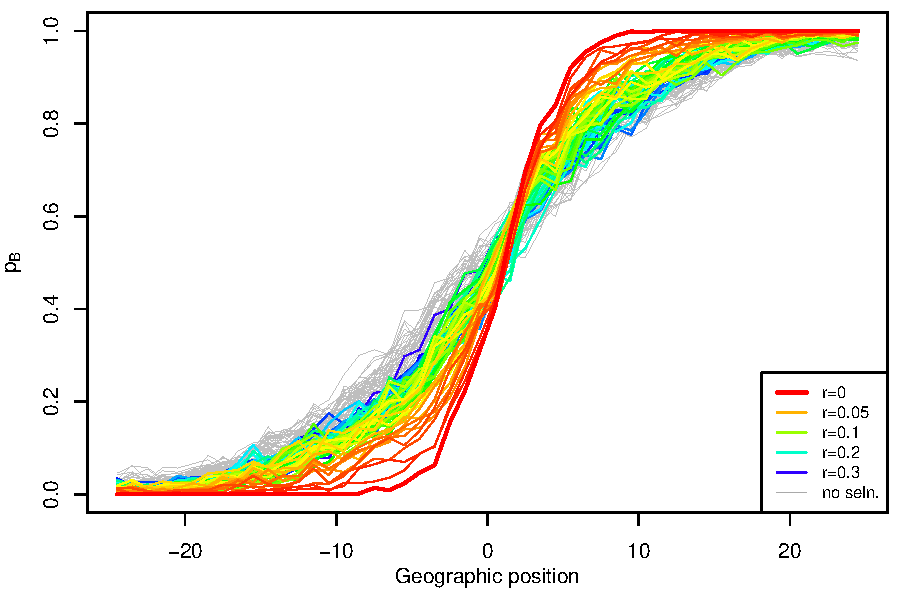
\includegraphics{{figs/alleleFrequencies_sim_s0.01_tau100_closely_linked}.pdf}
    \caption{
    Frequency of ancestry $B$,
    across geography at different physical positions on the genome, simulated for a hybrid zone
     $T=100$ generations after secondary contact, with $s=0.1$,
     using 50 demes, each with 500 diploid individuals and $\sigma=1$.
    Each line represents a locus some distance $r$ away from the true target of selection with colors corresponding to different values of $r$, transitioning from red (tight linkage to selected site) to blue (distantly linked).
    Grey lines represent the same positions from a simulation with
    identical parameters except that $s=0$. 
    Corresponding theoretical quantities are shown juxtaposed in Figure \ref{fig:alleleFreq_tau100_comparison};
    the same plot is shown with weaker selection in Figure \ref{alleleFreq_tau100_weaker_s} and at a longer time in Figure \ref{alleleFreq_tau1000}.
}\label{alleleFreq_tau100}
\end{figure}



\begin{figure}
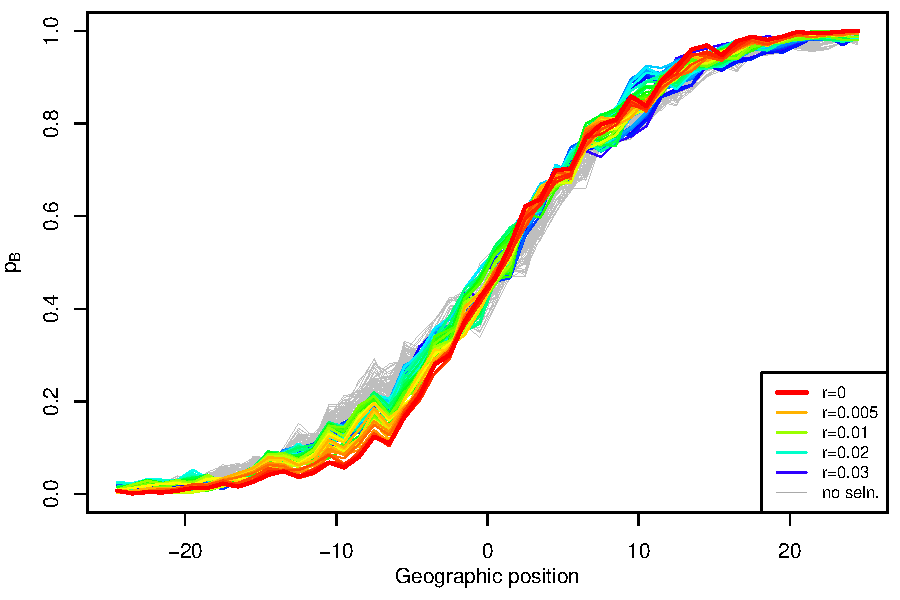
\includegraphics{figs/alleleFrequencies_sim_s01_tau100_closely_linked.pdf}
\caption{
    Frequency of ancestry $B$,
    across geography and at several physical positions on the genome, simulated for a hybrid zone
     $T=100$ generations after secondary contact,
    and with $s=0.01$.
    The simulated zone had 50 demes, each with a population size of 500 diploid individuals.
    Each line represents a locus some distance $r$ away from the true target of selection, 
    and $r=0$ represents the locus that is under selection. Grey lines represent the same positions from a simulation with
    identical parameters except that $s=0$.
}\label{alleleFreq_tau100_weaker_s}
\end{figure}

\begin{figure}
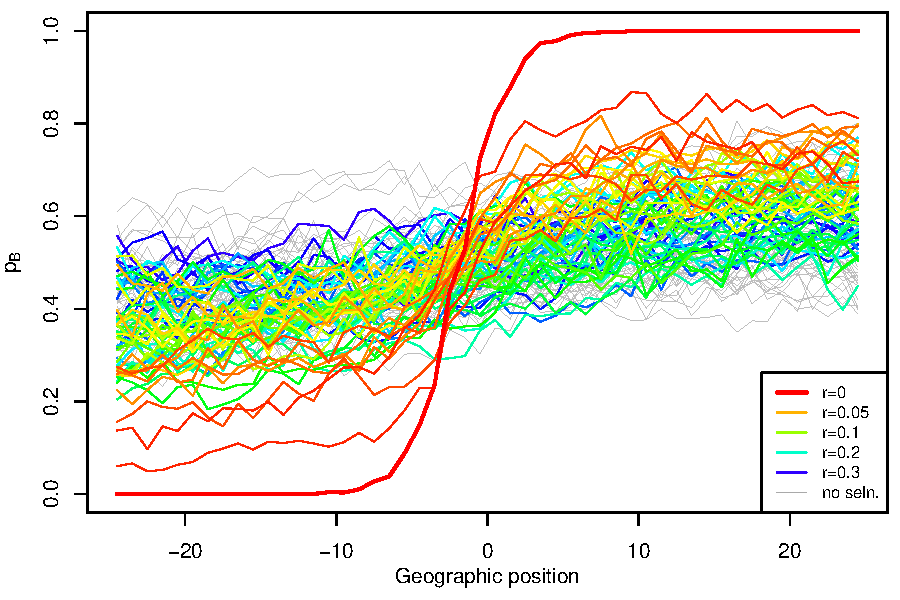
\includegraphics{figs/alleleFrequencies_sim_s1_tau1000.pdf}
\caption{
    Frequency of ancestry $B$,
    across geography and at several physical positions on the genome, simulated for a hybrid zone
     $T=1000$ generations after secondary contact,
    and with $s=0.1$.
    The simulated zone had 50 demes, each with a population size of 500 diploid individuals.
    Each line represents a locus some distance $r$ away from the true target of selection, 
    and $r=0$ represents the locus that is under selection. Grey lines represent the same positions from a simulation with
    identical parameters except that $s=0$.
 }\label{alleleFreq_tau1000}
\end{figure}

\begin{figure}
    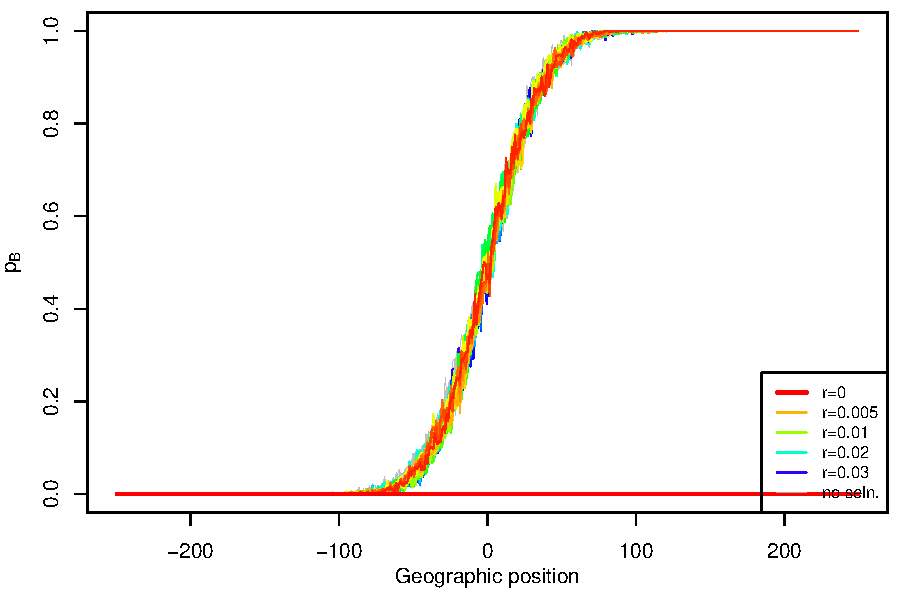
\includegraphics{{figs/alleleFrequencies_sim_SIGMA3_Ninds250000_ndemes500_s0.01_tau100}.pdf}
\caption{
    Frequency of ancestry $B$,
    across geography and at several physical positions on the genome, simulated for a hybrid zone
    $T=100$ generations after secondary contact,
    and with $s=0.01$.
    The simulated zone had 500 demes, each with a population size of 500 diploid individuals.
    Each line represents a locus some distance $r$ away from the true target of selection, 
    and $r=0$ represents the locus that is under selection. Grey lines represent the same positions from a simulation with
    identical parameters except that $s=0$.
}\label{sfig:extra_long_cline}
\end{figure}



\begin{figure}
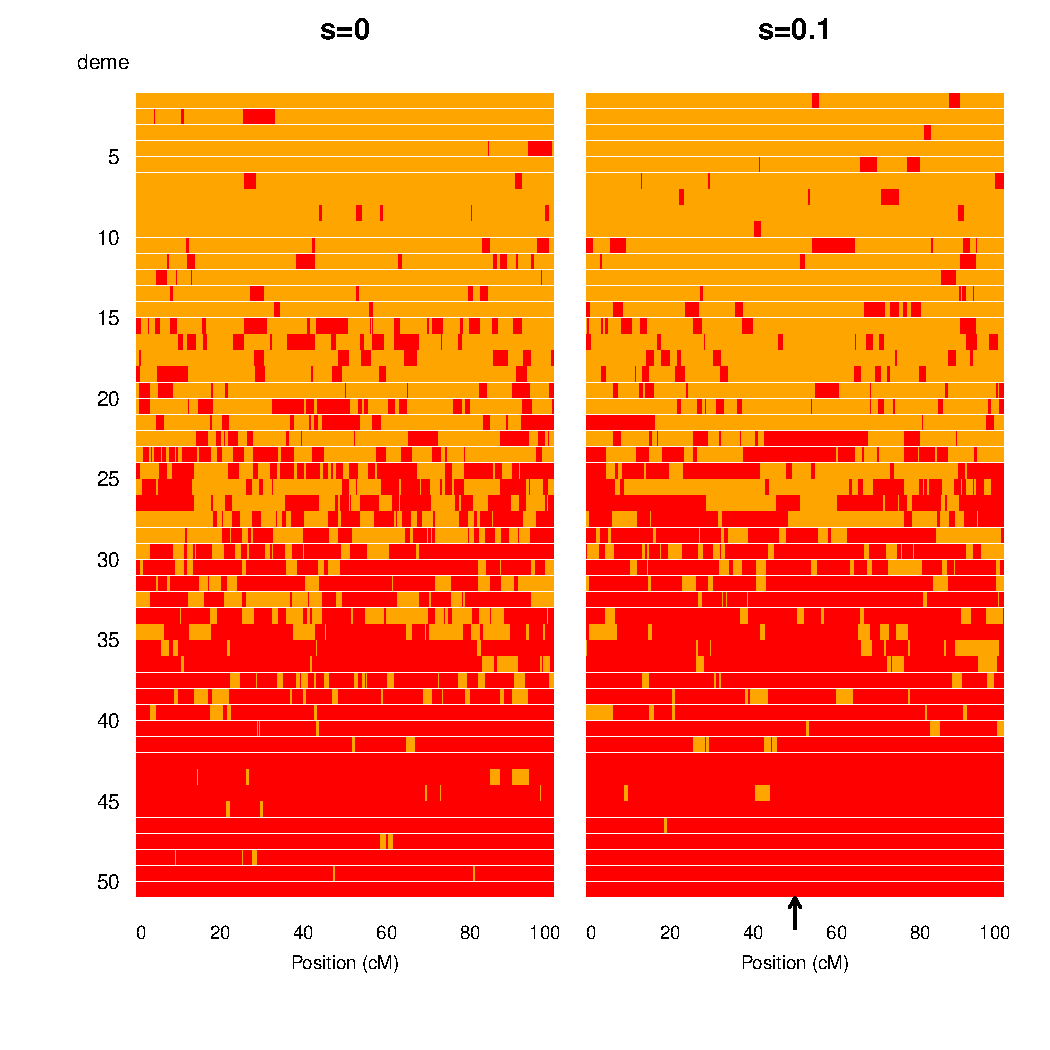
\includegraphics[width=\textwidth]{figs/plot_chromosomes_tau100.pdf}
\caption{Randomly sampled chromosomes  across a hybrid zone of age $T=100$. Here we compare chromosomes of length 1M from a neutral zone to one that has a single under-dominant locus ($s=0.1$) in the middle of the chromosome (indicated by black arrow). Red blocks along the chromosome denote ancestry $B$, and orange blocks are ancestry $A$.
 }\label{Fig:resistanceToIntrogression100g}
\end{figure}


\begin{figure}
    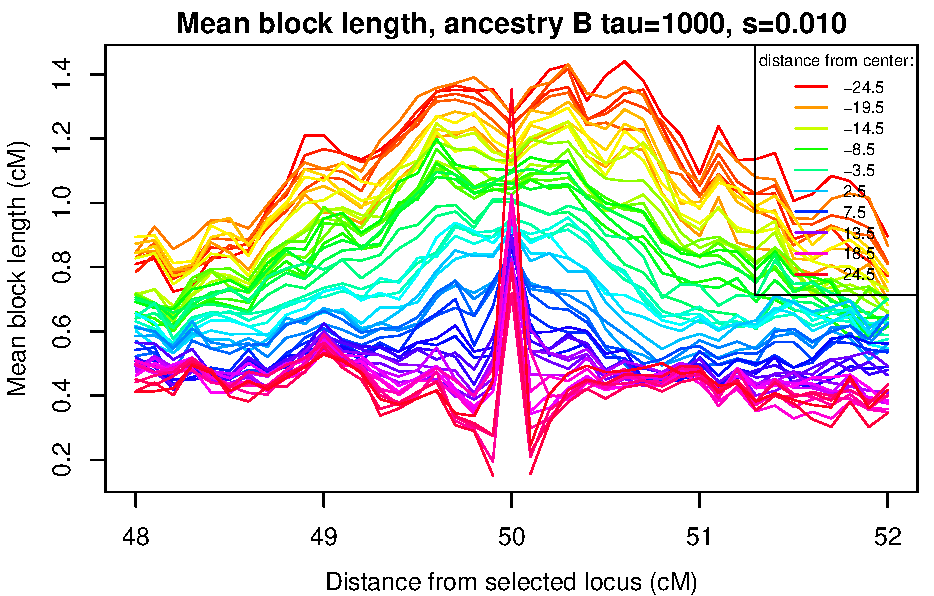
\includegraphics{{figs/simulation_SIGMA1_Ninds25000_ndemes50_s0.01_tau1000_blocksAlongChromAncBConditioning_nonnormalized}.pdf}
    \caption{
        \textbf{Mean haplotype lengths of $B$ haplotypes}, $l_B(x,m)$,
        across the genome (horizontal axis) and at different spatial locations (colored lines),
        from a simulation with 50 demes having 500 individuals each, $s=0.01$, $\sigma=1$, and after $T=1000$ generations.
    } \label{sfig:blocksAlongChromAncBConditioning_nonnormalized}
\end{figure}

\begin{figure}
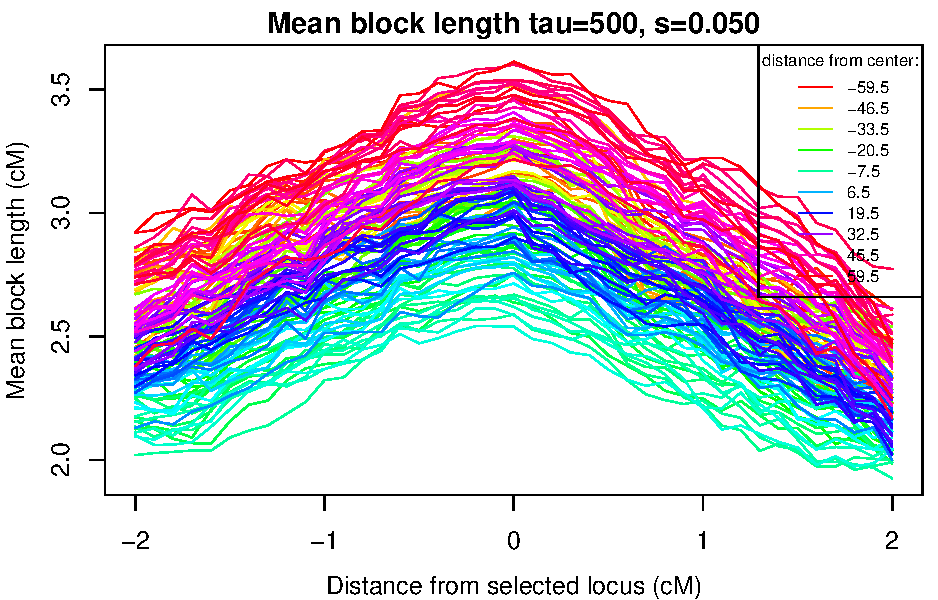
\includegraphics[width=\textwidth]{{figs/results_runid_753324_chr1_start0.48_stop0.52_by0.001_blocksAlongChromNoConditioning_nonnormalized}.pdf}
\caption{
    \textbf{Mean enclosing block length $l(m,x)$}, across the genome (horizontal axis)
    and at different geographic positions (different colored lines).
    Results are from a simulation with 120 demes of 200 diploids each, selection $s=.05$, dispersal $\sigma=3$, 
    and after $T=500$ generations.
}\label{Fig:meanBlockLengthsUnconditioned}
\end{figure}


\begin{figure}
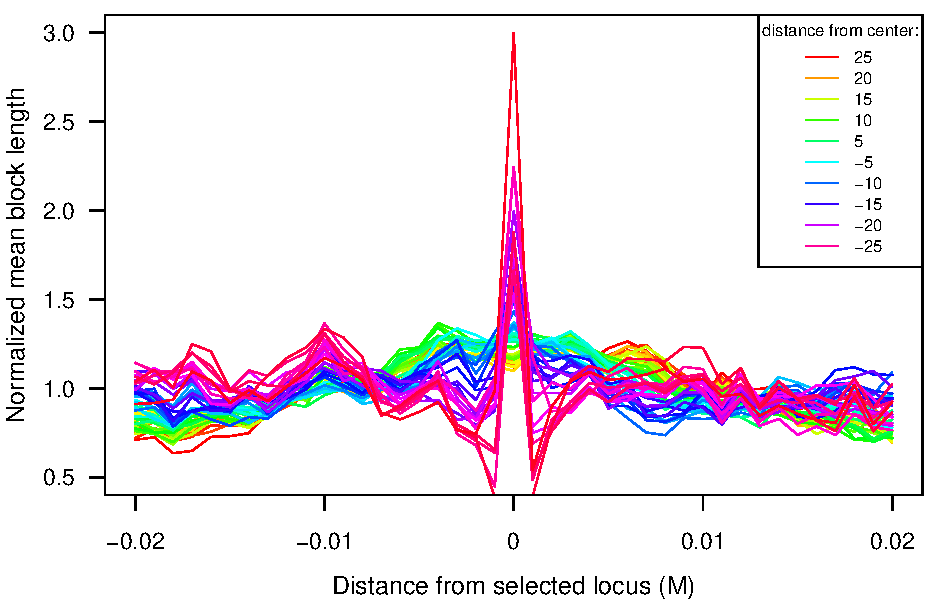
\includegraphics{figs/blocksAlongChromAncBConditioning.pdf}
\caption{
    \textbf{Normalized mean enclosing block length}, $\bar l_B(m,x)$, after $T=1000$ generations,
    against position relative to the selected locus (horizontal axis)
    located in the center of a 1M chromosome.
    Each line shows the mean block length at that spatial and genomic position
    divided by the mean over the chromosome at that location;
    the simulation was run with $s=0.01$ and $\sigma=1$,
    50 demes, each containing 500 diploid individuals.
}\label{Fig:blockLengths}
\end{figure}


\begin{figure}
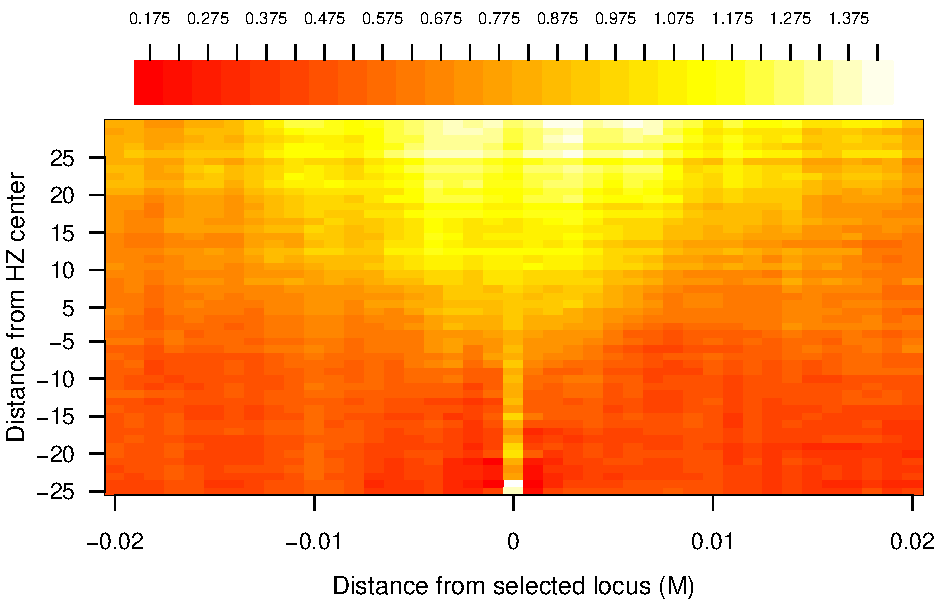
\includegraphics{figs/blocksAlongChromHeatmapAncBConditioning.pdf}
\caption{Heatmap of mean block length $l_B(m)$ along a simulated chromosome under $T=1000$, $s=0.01$ and $\sigma=1$,
    50 demes, each containing 500 diploid individuals. }\label{Supp:blockLengthHeatmap}
\end{figure}




\begin{figure}
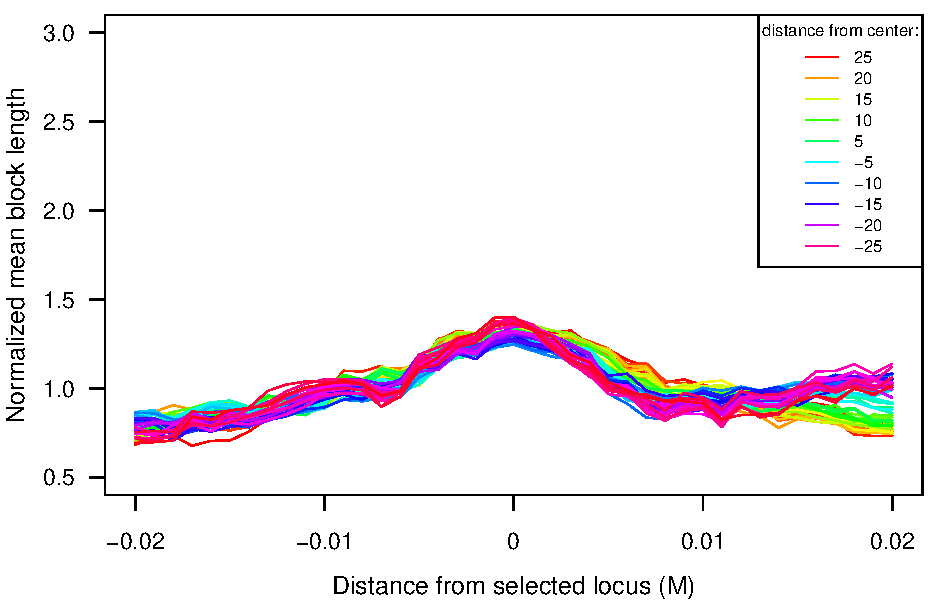
\includegraphics{figs/blocksAlongChromNoConditioning.pdf}
\caption{Mean block length $l(m)$, without conditioning on ancestry, surrounding a given position along the genome with a single underdominant site with parameters as for Fig~\ref{Fig:blockLengths}. ($s=0.01, T=1000, \sigma=1$). }\label{Supp:blockLengthNoAnc}
\end{figure}

\begin{figure}
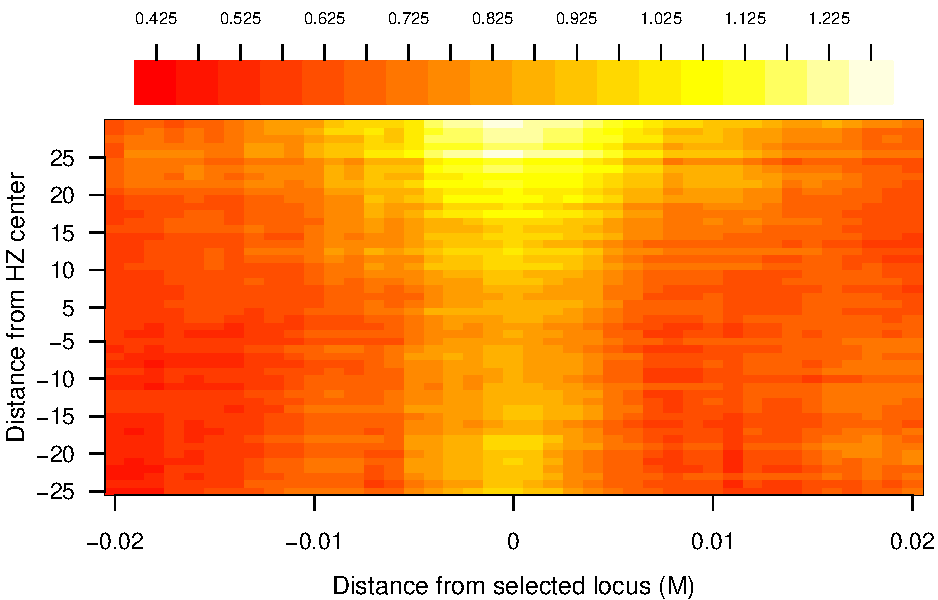
\includegraphics{figs/blocksAlongChromHeatmap.pdf}
\caption{Heatmap of mean block length $l(m)$, without conditioning on ancestry, along a simulated chromosome with a single underdominant site, with parameters as for Fig~\ref{Fig:blockLengths} ($s=0.01, T=1000, \sigma=1$) }\label{Supp:blockLengthHeatmapNoAnc}
\end{figure}


\begin{figure}
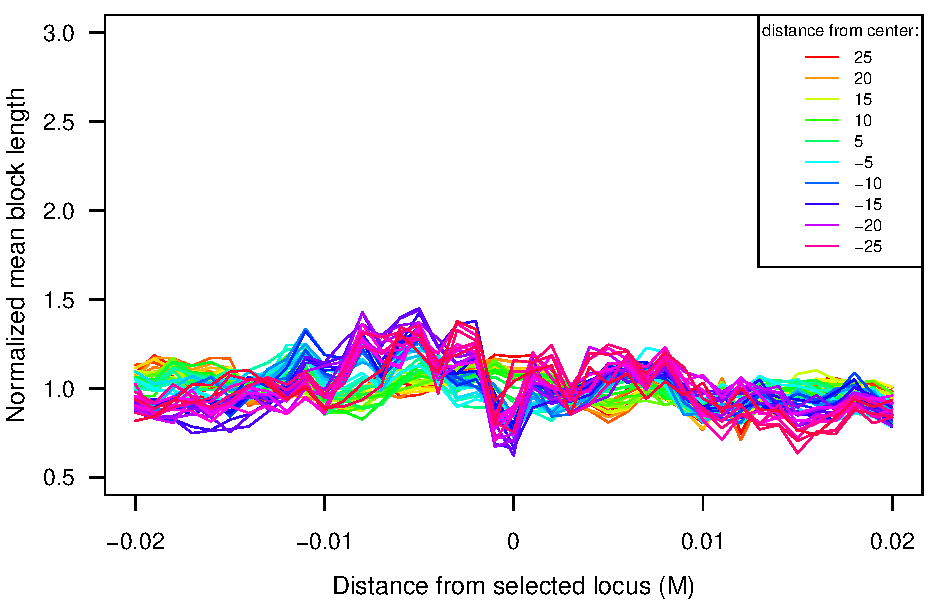
\includegraphics{figs/adjacentBlocksAlongChromAncBConditioning.pdf}
\caption{Mean block length of $l_A(m\pm)$ across chromosome with single under dominant site, conditioning on ancestry $B$ at the selected locus, with parameters as for Fig~\ref{Fig:blockLengths} ($s=0.01, T=1000, \sigma=1$)}\label{Supp:adjacentBlocks}
\end{figure}


\begin{figure}
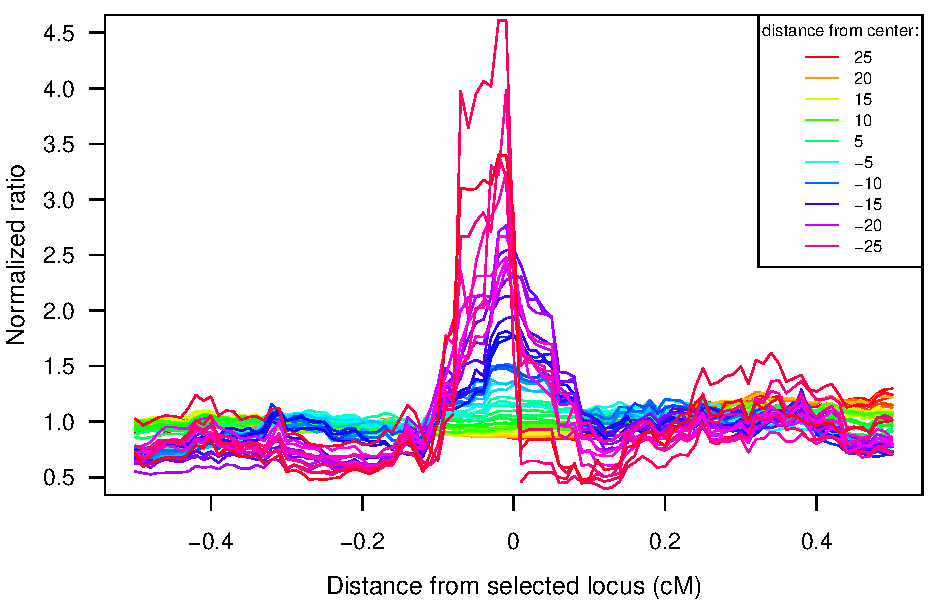
\includegraphics{figs/s0point01_ratioAdjacentBlocksAlongChromAncBConditioningHighRes.pdf}
    \caption{The normalized statistic $\bar C(m,x)$: the ratio $\frac{2\sum{l_B(m_i)}}{\sum{l_A(m_i-)+I_A(m_i+)}}$ of mean block length and mean adjacent block lengths across a simulated chromosome with a single underdominant site and conditioning on ancestry $B$ at the selected site ($s=0.01, T=1000$).  Each line represents a deme and is normalized by mean block length across the chromosome in the deme. This  simulation corresponds to that represented in Figure~\ref{Fig:blockLengthsZoom}; note the difference in y-axis scale.}\label{Supp:ratioBlockAdjacent}
\end{figure}


\begin{figure}
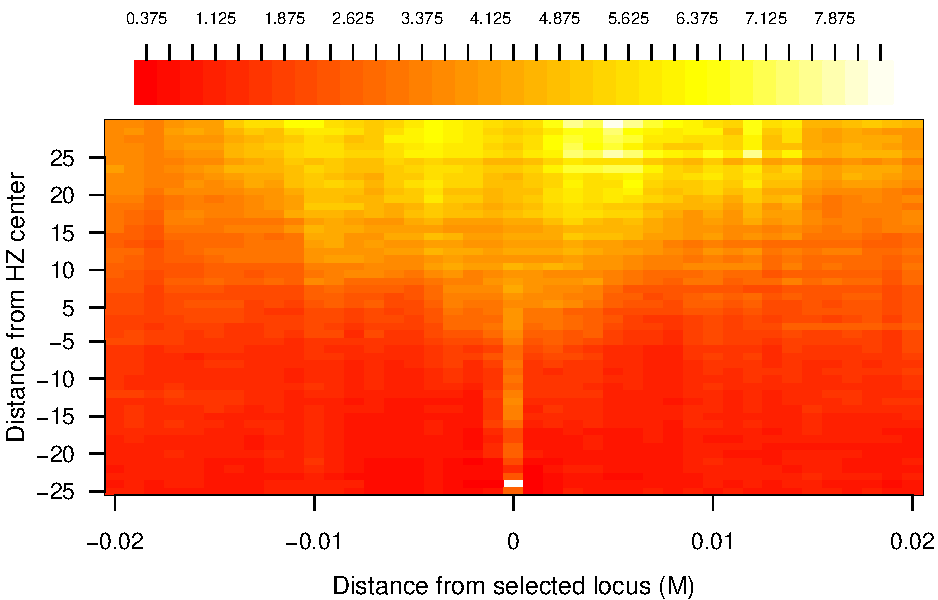
\includegraphics{figs/ratioAdjacentBlocksAlongChromHeatmapAncBConditioning.pdf}
    \caption{Heatmap of $C(m,x)=\frac{2\sum{l_B(m_i)}}{\sum{l_A(m_i-)+I_A(m_i+)}}$ across a simulated chromosome with a single underdominant site and conditioning on ancestry $B$ at the selected site and parameters as for Fig.~\ref{Fig:blockLengths} ($s=0.01, T=1000, \sigma=1$). }\label{Supp:ratioBlockAdjacentHeatmap}
\end{figure}


\begin{figure}
    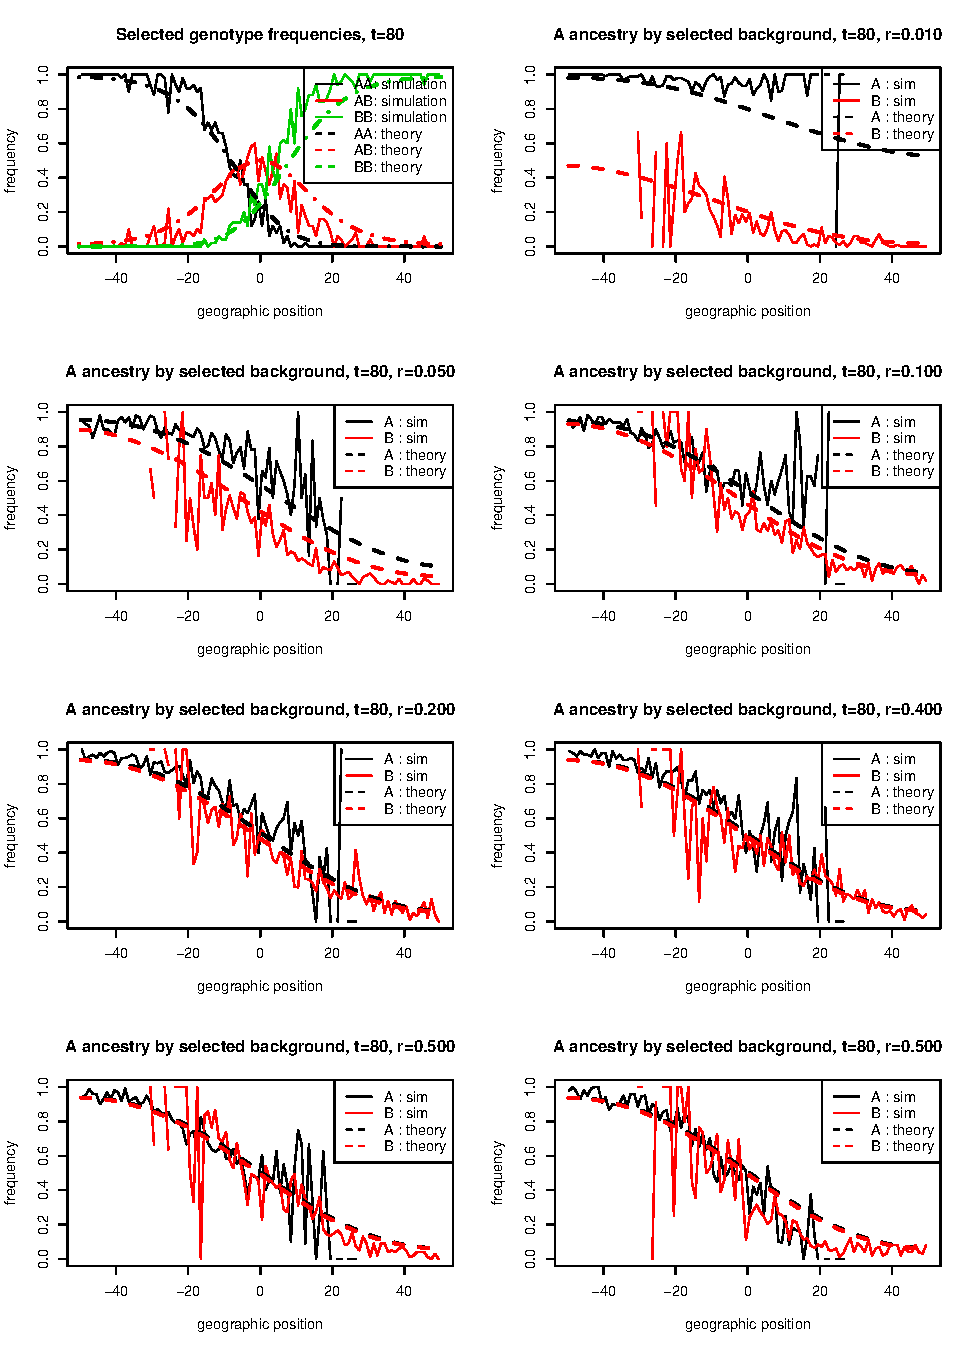
\includegraphics[height=0.8\textheight]{figs/cond_freqs_comparison_tau_80.pdf}
    \caption{
        \textbf{Conditional frequencies of ancestry $A$ at $\tau=80$},
        comparing simulation and theory, with $\sigma=3$ deme spacings, $s=0.05$, and 50 individuals per deme.
        The top left figure shows observed and expected genotype frequencies for the two homozygotes and the heterozygote at the selected locus;
        expected genotype counts were obtained assuming random mating,
        and by solving equation \eqref{eqn:cline_pde} numerically.
        The remaining figures show observed and expected frequencies of $A$ ancestry,
        separately conditioned on the identity of the linked allele at the selected site.
        Observed frequencies become much noisier where the linked allele becomes rarer.
    } \label{sfig:condAlleleFreq_tau80_comparison}
\end{figure}


\begin{figure}
    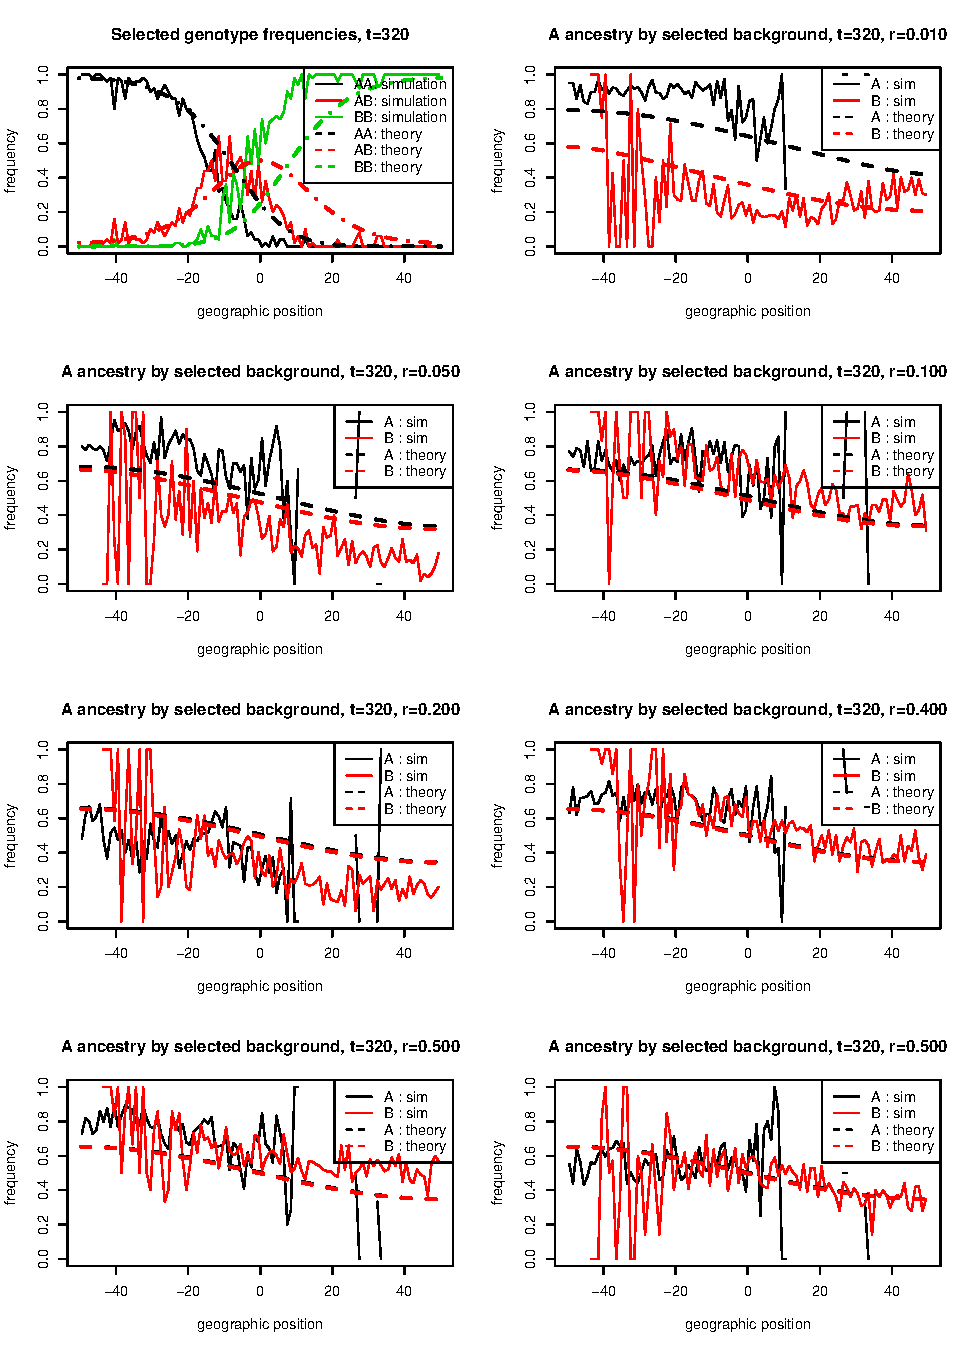
\includegraphics{figs/cond_freqs_comparison_tau_320.pdf}
    \caption{
        \textbf{Conditional frequencies of ancestry $A$ at $\tau=320$},
        as in figure \ref{sfig:condAlleleFreq_tau80_comparison}.
        Deviations are larger than at $\tau=80$, 
        due to genetic drift.
    } \label{sfig:condAlleleFreq_tau320_comparison}
\end{figure}


\begin{figure}
    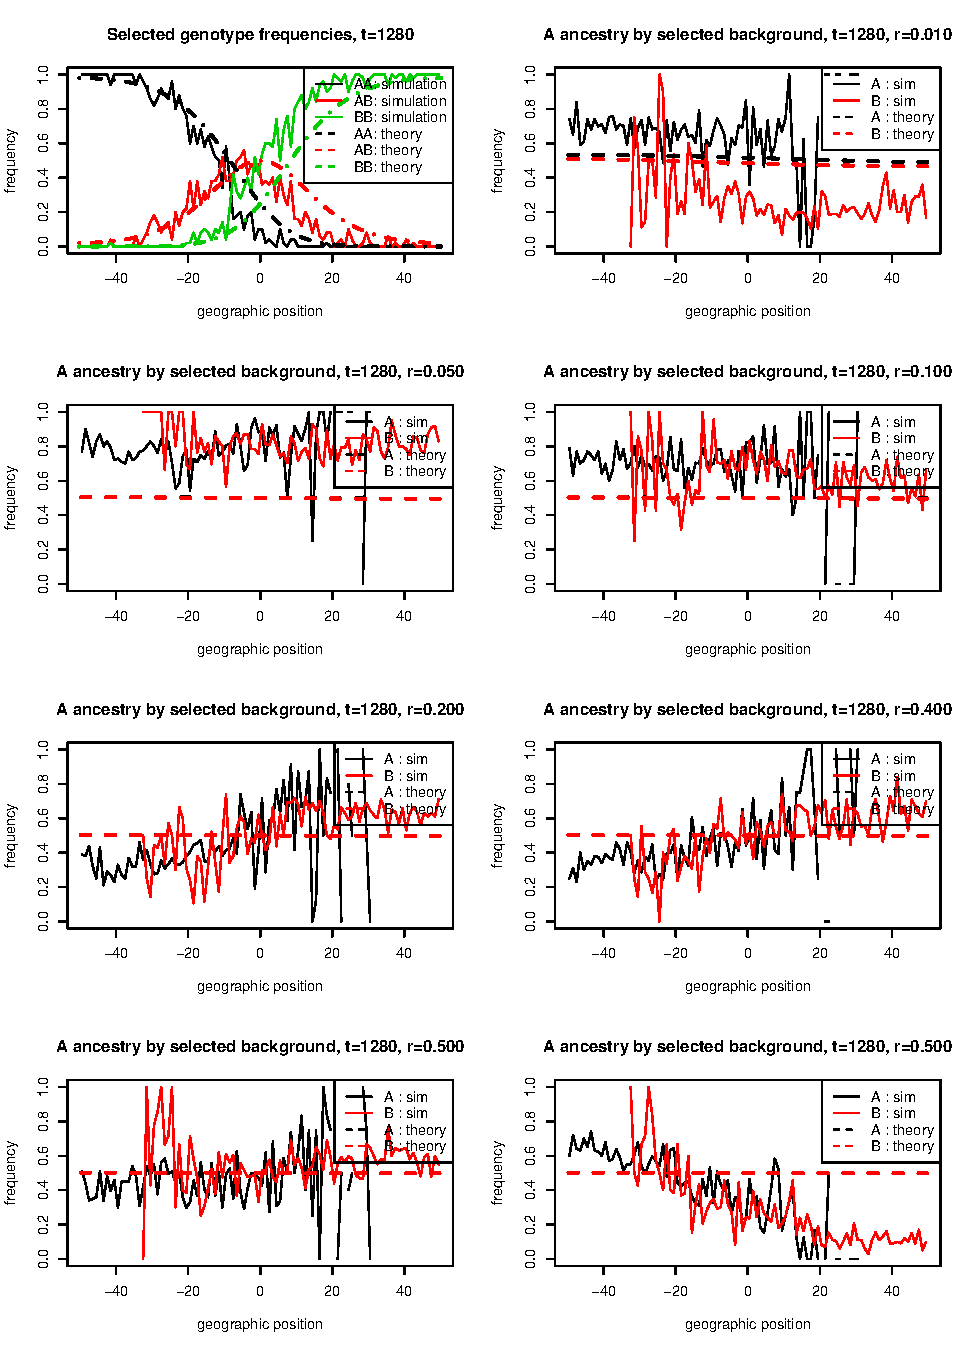
\includegraphics{figs/cond_freqs_comparison_tau_1280.pdf}
    \caption{
        \textbf{Conditional frequencies of ancestry $A$ at $\tau=1280$},
        as in figure \ref{sfig:condAlleleFreq_tau80_comparison}.
        Deviations are larger still than at $\tau=320$, 
        due to genetic drift.
    } \label{sfig:condAlleleFreq_tau1280_comparison}
\end{figure}
\clearpage
\begin{figure}
    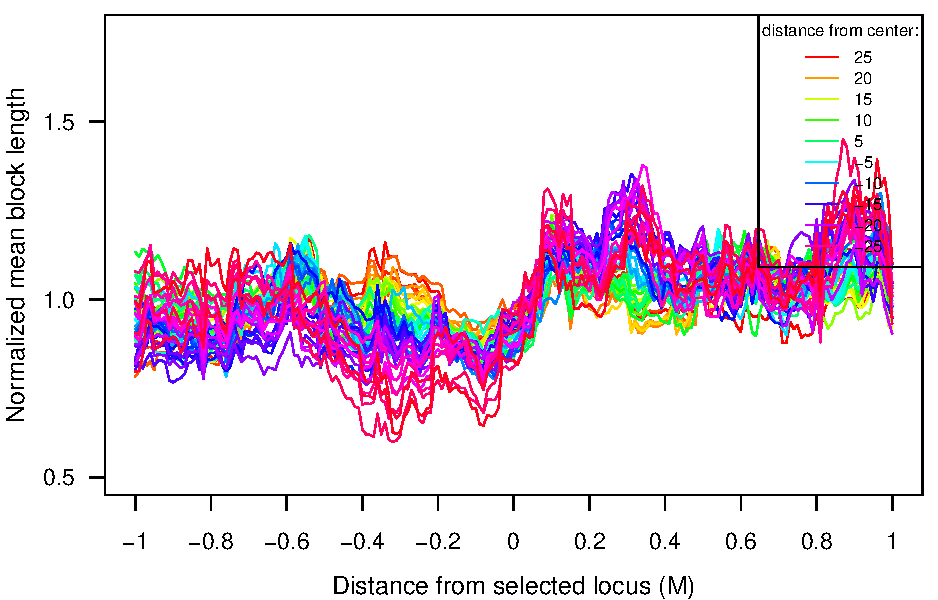
\includegraphics{figs/s001_adjacentBlocksAlongChromAncBConditioning}
    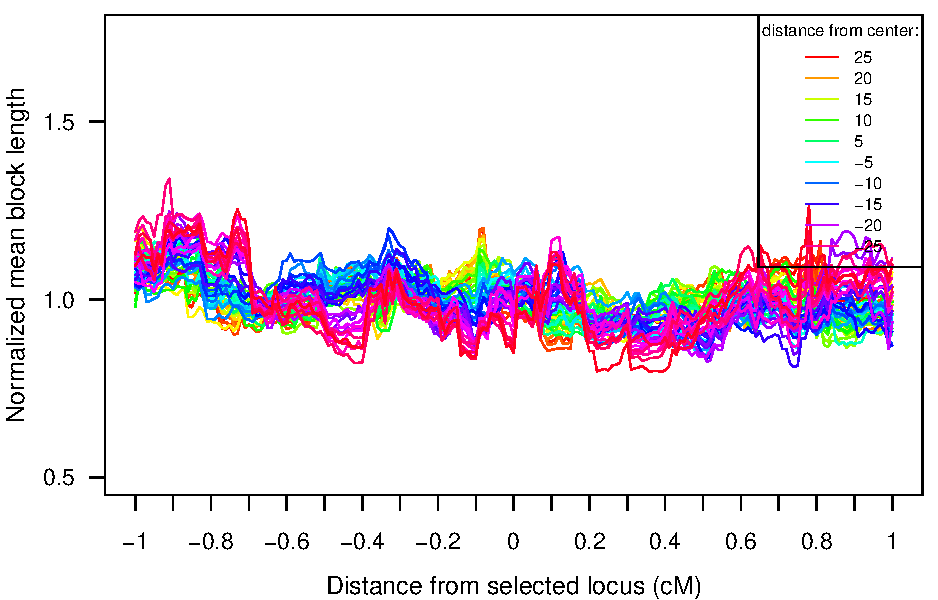
\includegraphics{figs/s001_adjacentBlocksAlongChromNoConditioningHighRes}
        \caption{
     Normalized ancestry $B$ block lengths (top) and all ancestry block lengths (bottom) along chromosome under $s=0.001$ and other parameters as for Fig.~\ref{Fig:blockLengths} ($\tau=1000,\sigma=1$). } \label{sfig:blockLengthPlot_t1000_s0.001}
\end{figure}


% \end{document}


%% response to reviews
% to remove these, change 'ifreviewresponses' up top
\singlespacing
\includereviews

\end{document}
